\subsection{Additional Time Series Analysis}
\label{appx-a:ch1:additional-time-series-analysis}

Since the plots in Section~\ref{ch1:subsec:time-series-analysis} are averages over a 10 minute moving average window (in order to aid visual representation of the volatile data), the raw and unfiltered data is included for reference in this appended section.

\begin{figure}\centering
\subfloat[Voltage levels as measured at the substation]{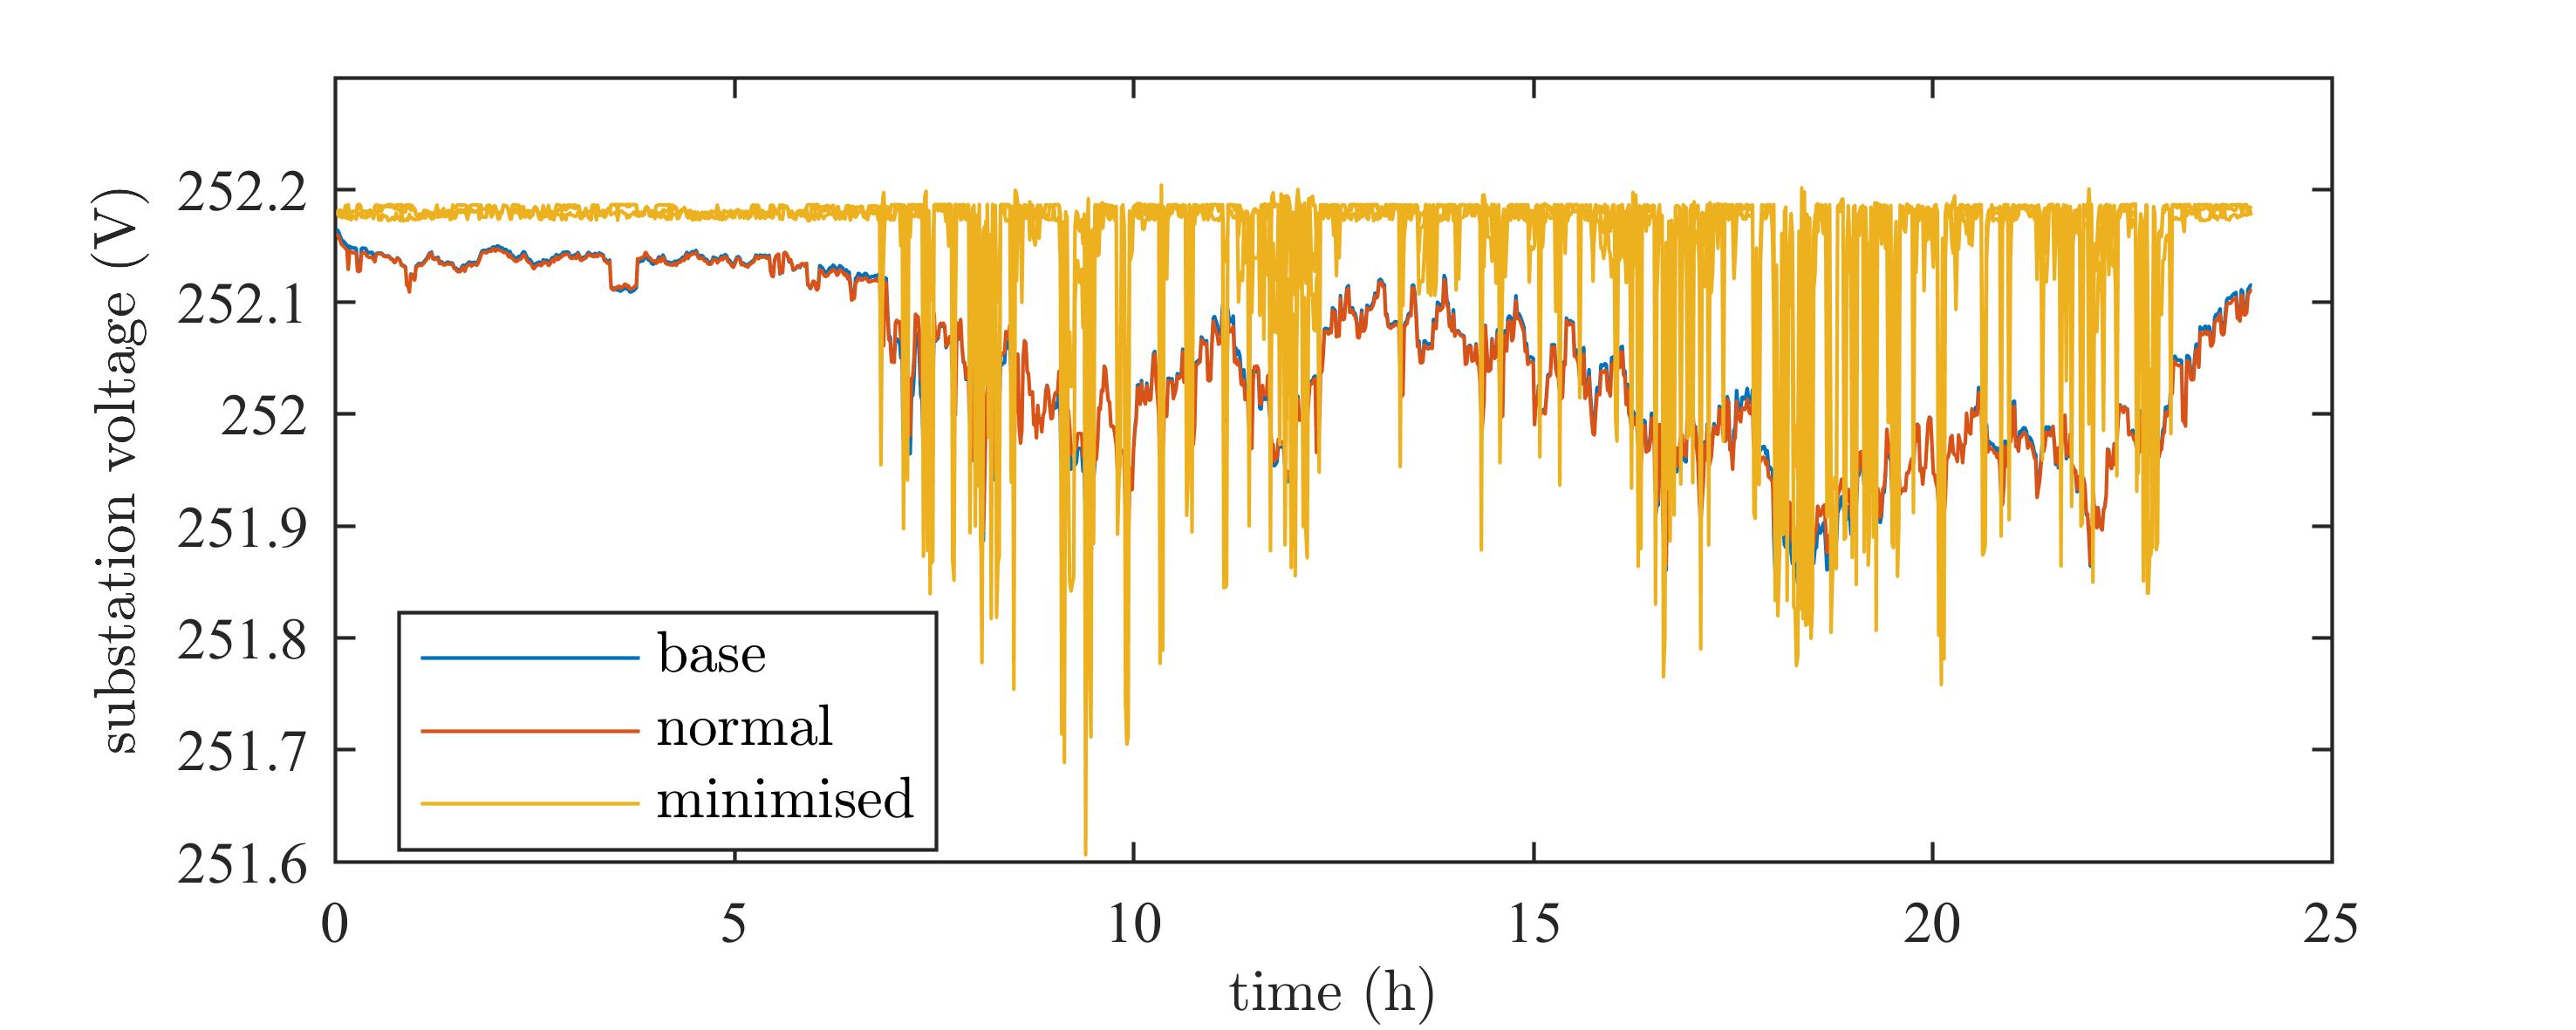
\includegraphics{_chapter1/fig/appendix/ts-substation-voltages___}}\\	
\subfloat[Cost associated with the voltage levels as measured at the substation]{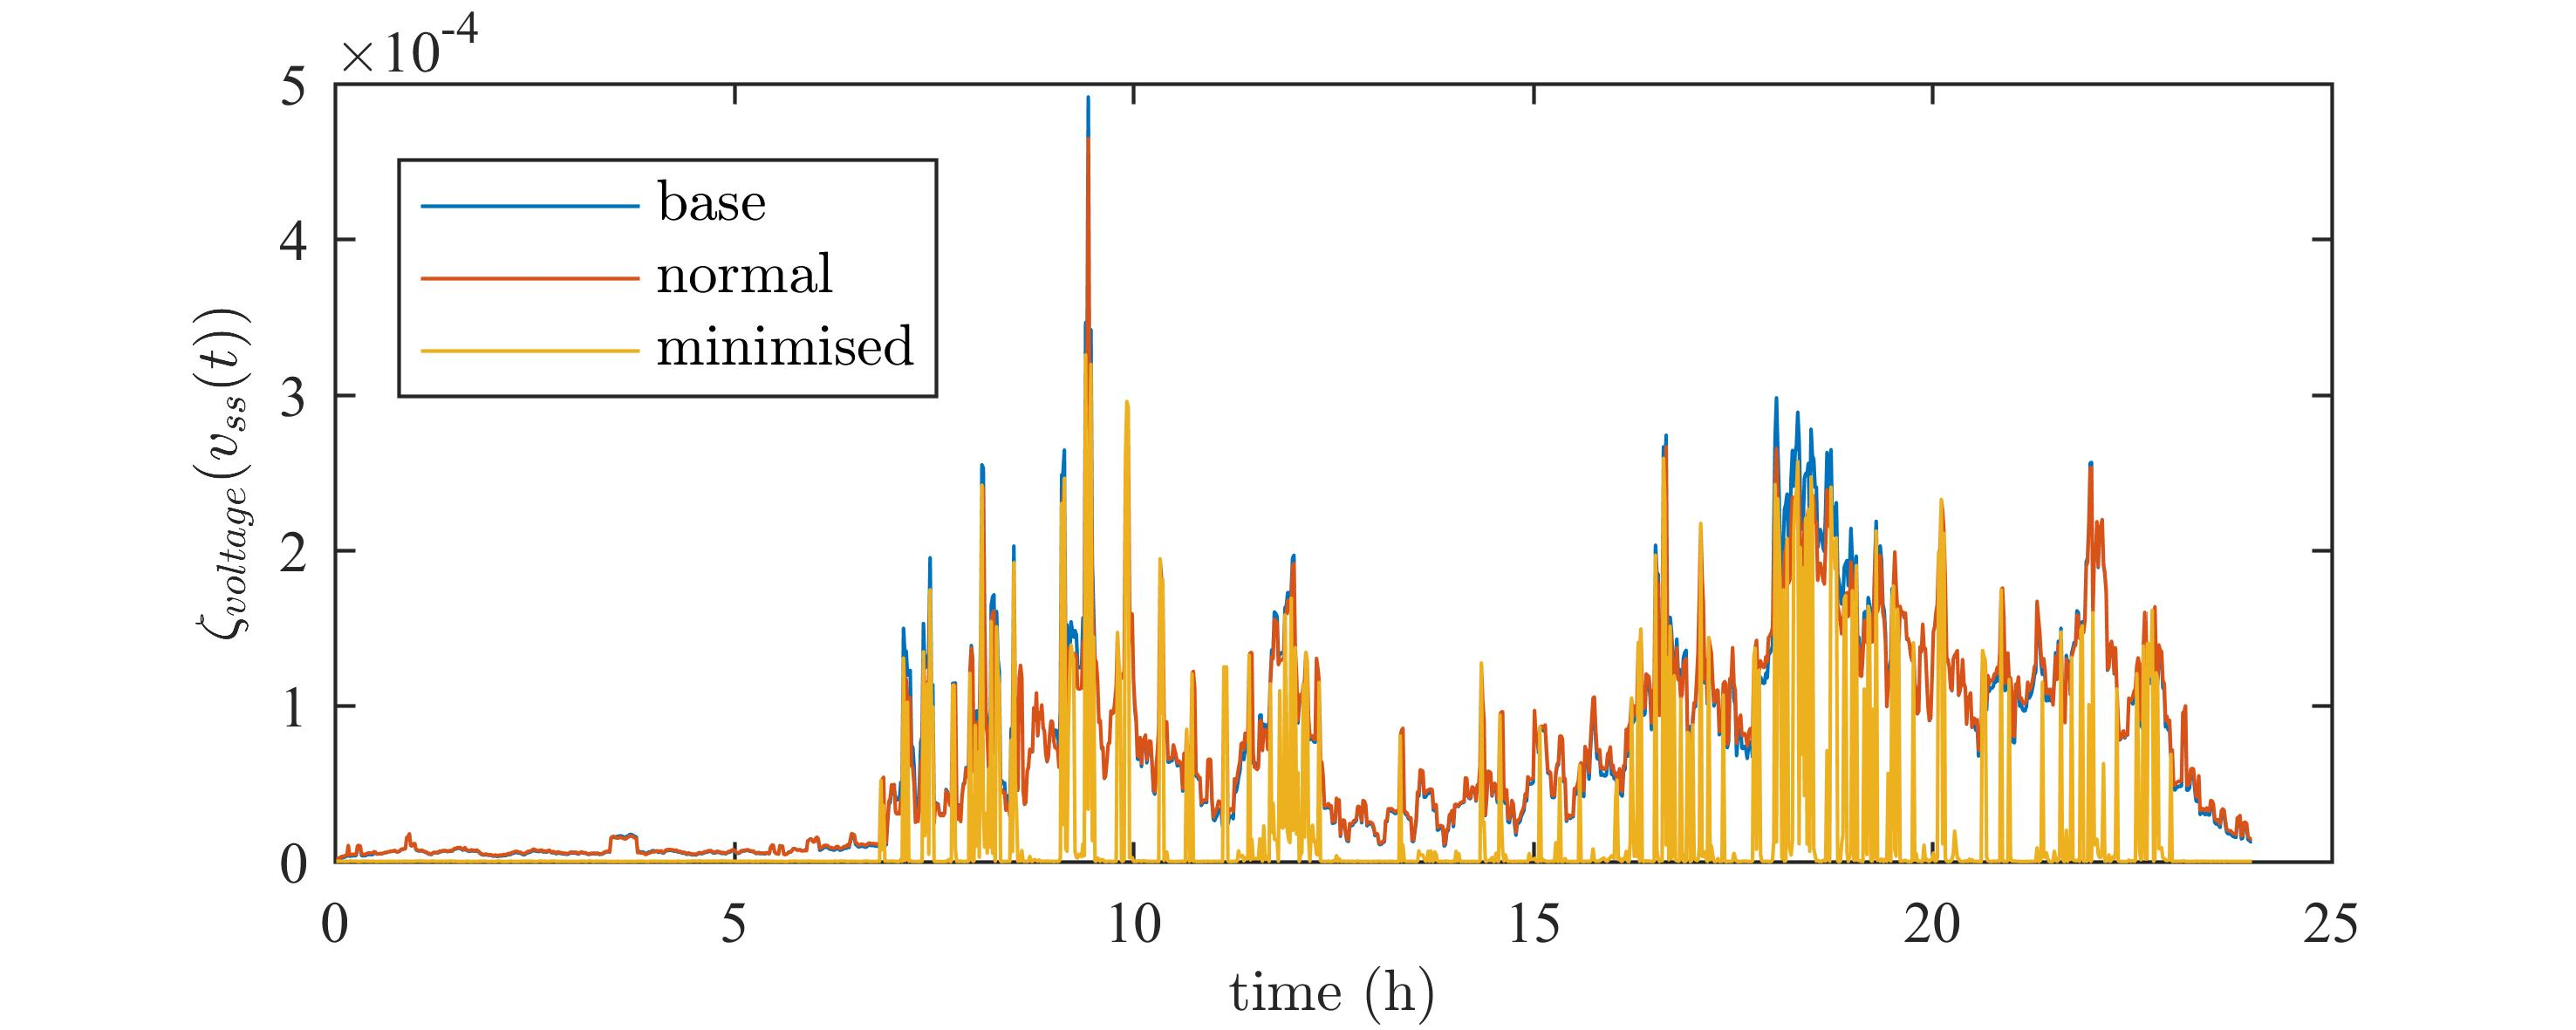
\includegraphics{_chapter1/fig/appendix/ts-substation-voltages__}}
\caption{Additional substation voltage level comparison between base, normal and the case where the ESMU's schedule was adjusted.}
\end{figure}

\begin{figure}\centering
\subfloat[ESMU voltage levels]{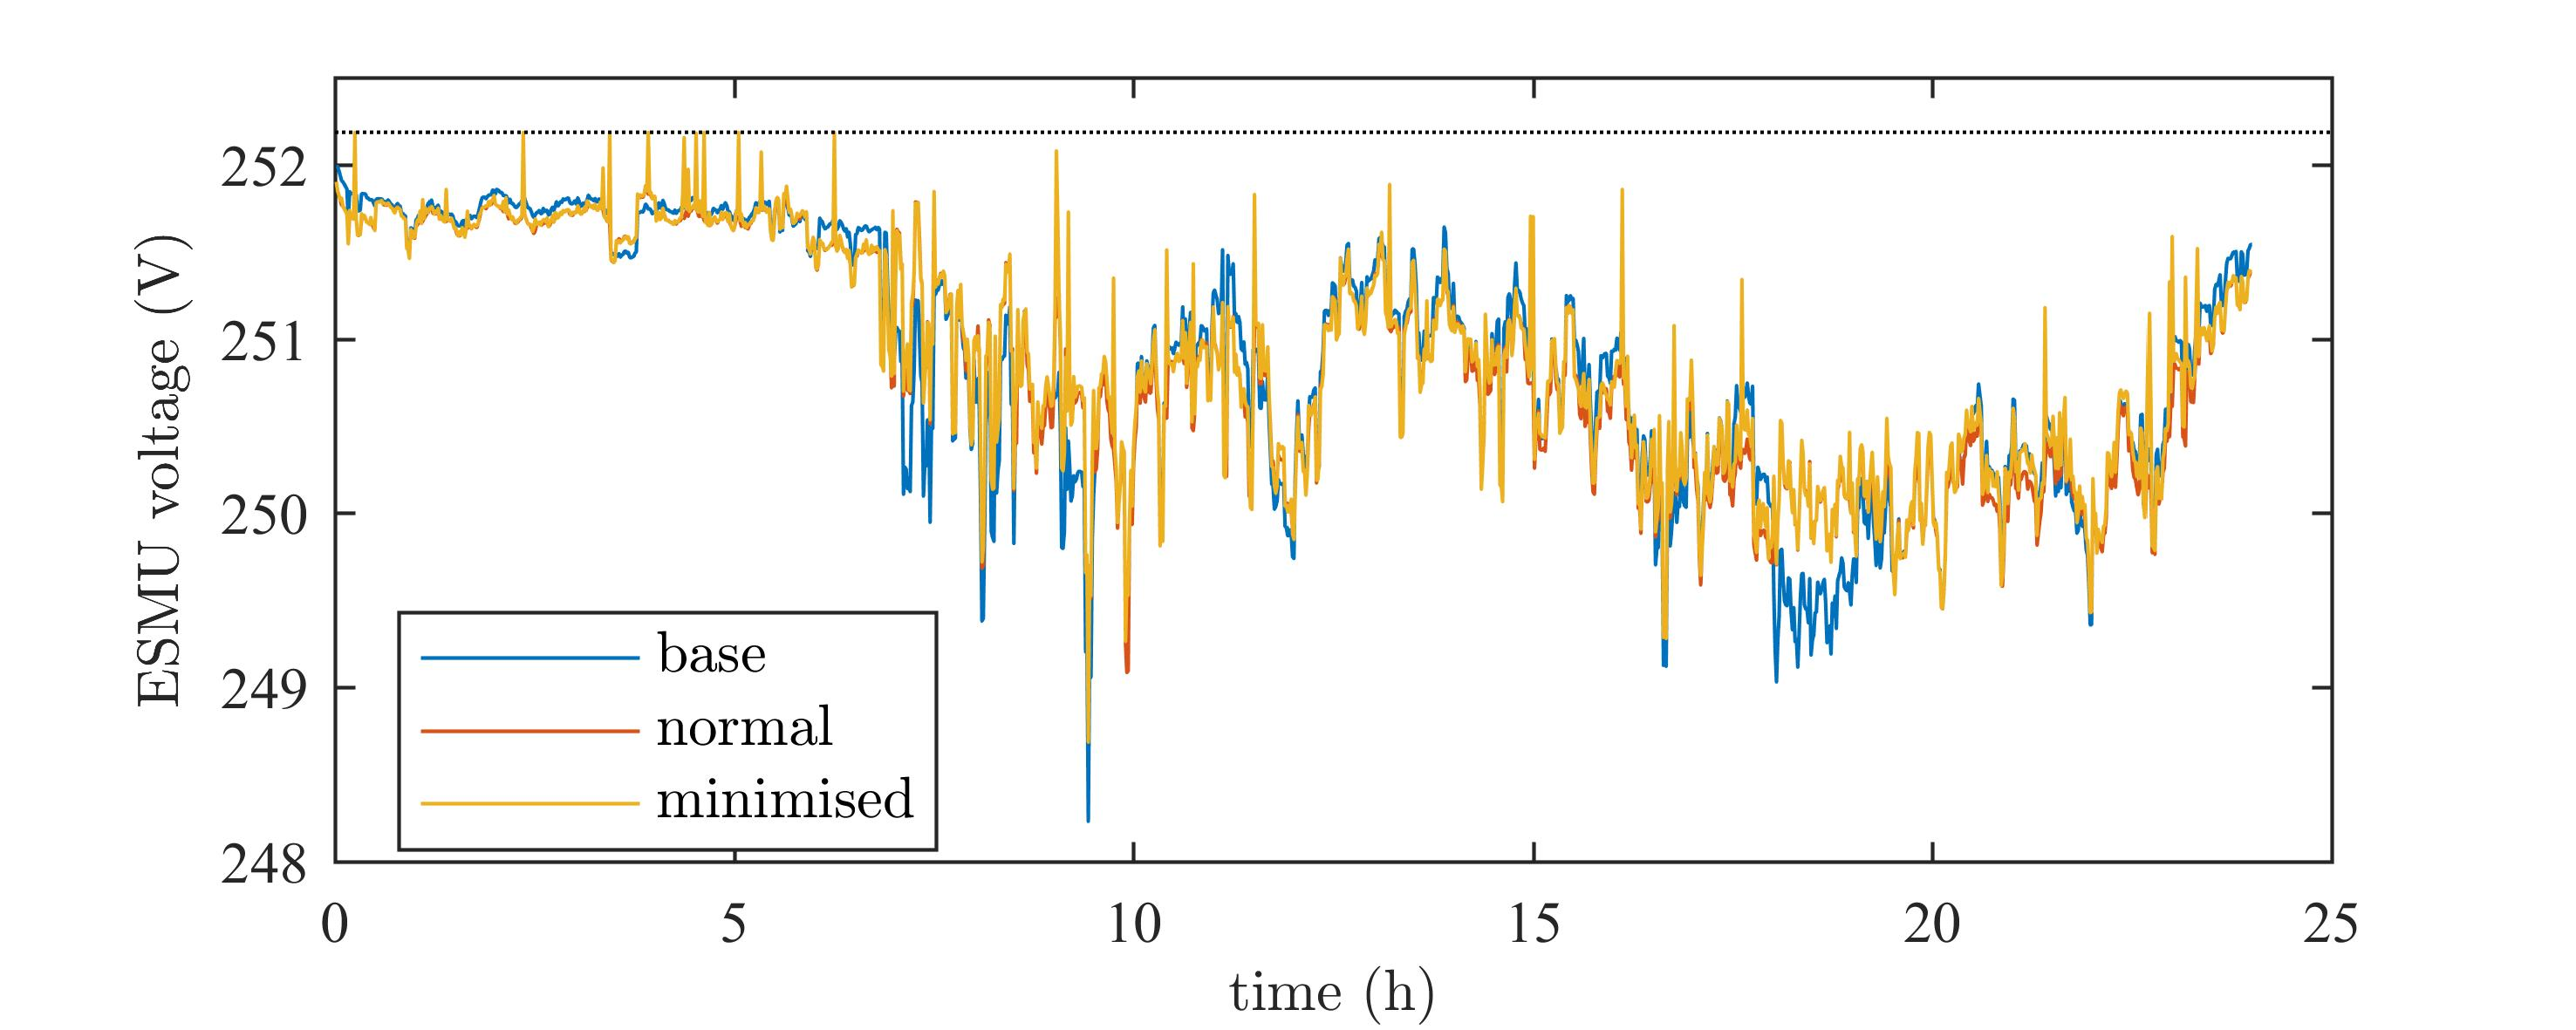
\includegraphics{_chapter1/fig/appendix/ts-esmu-voltages___}}\\	
\subfloat[Cost associated with the ESMU voltage levels]{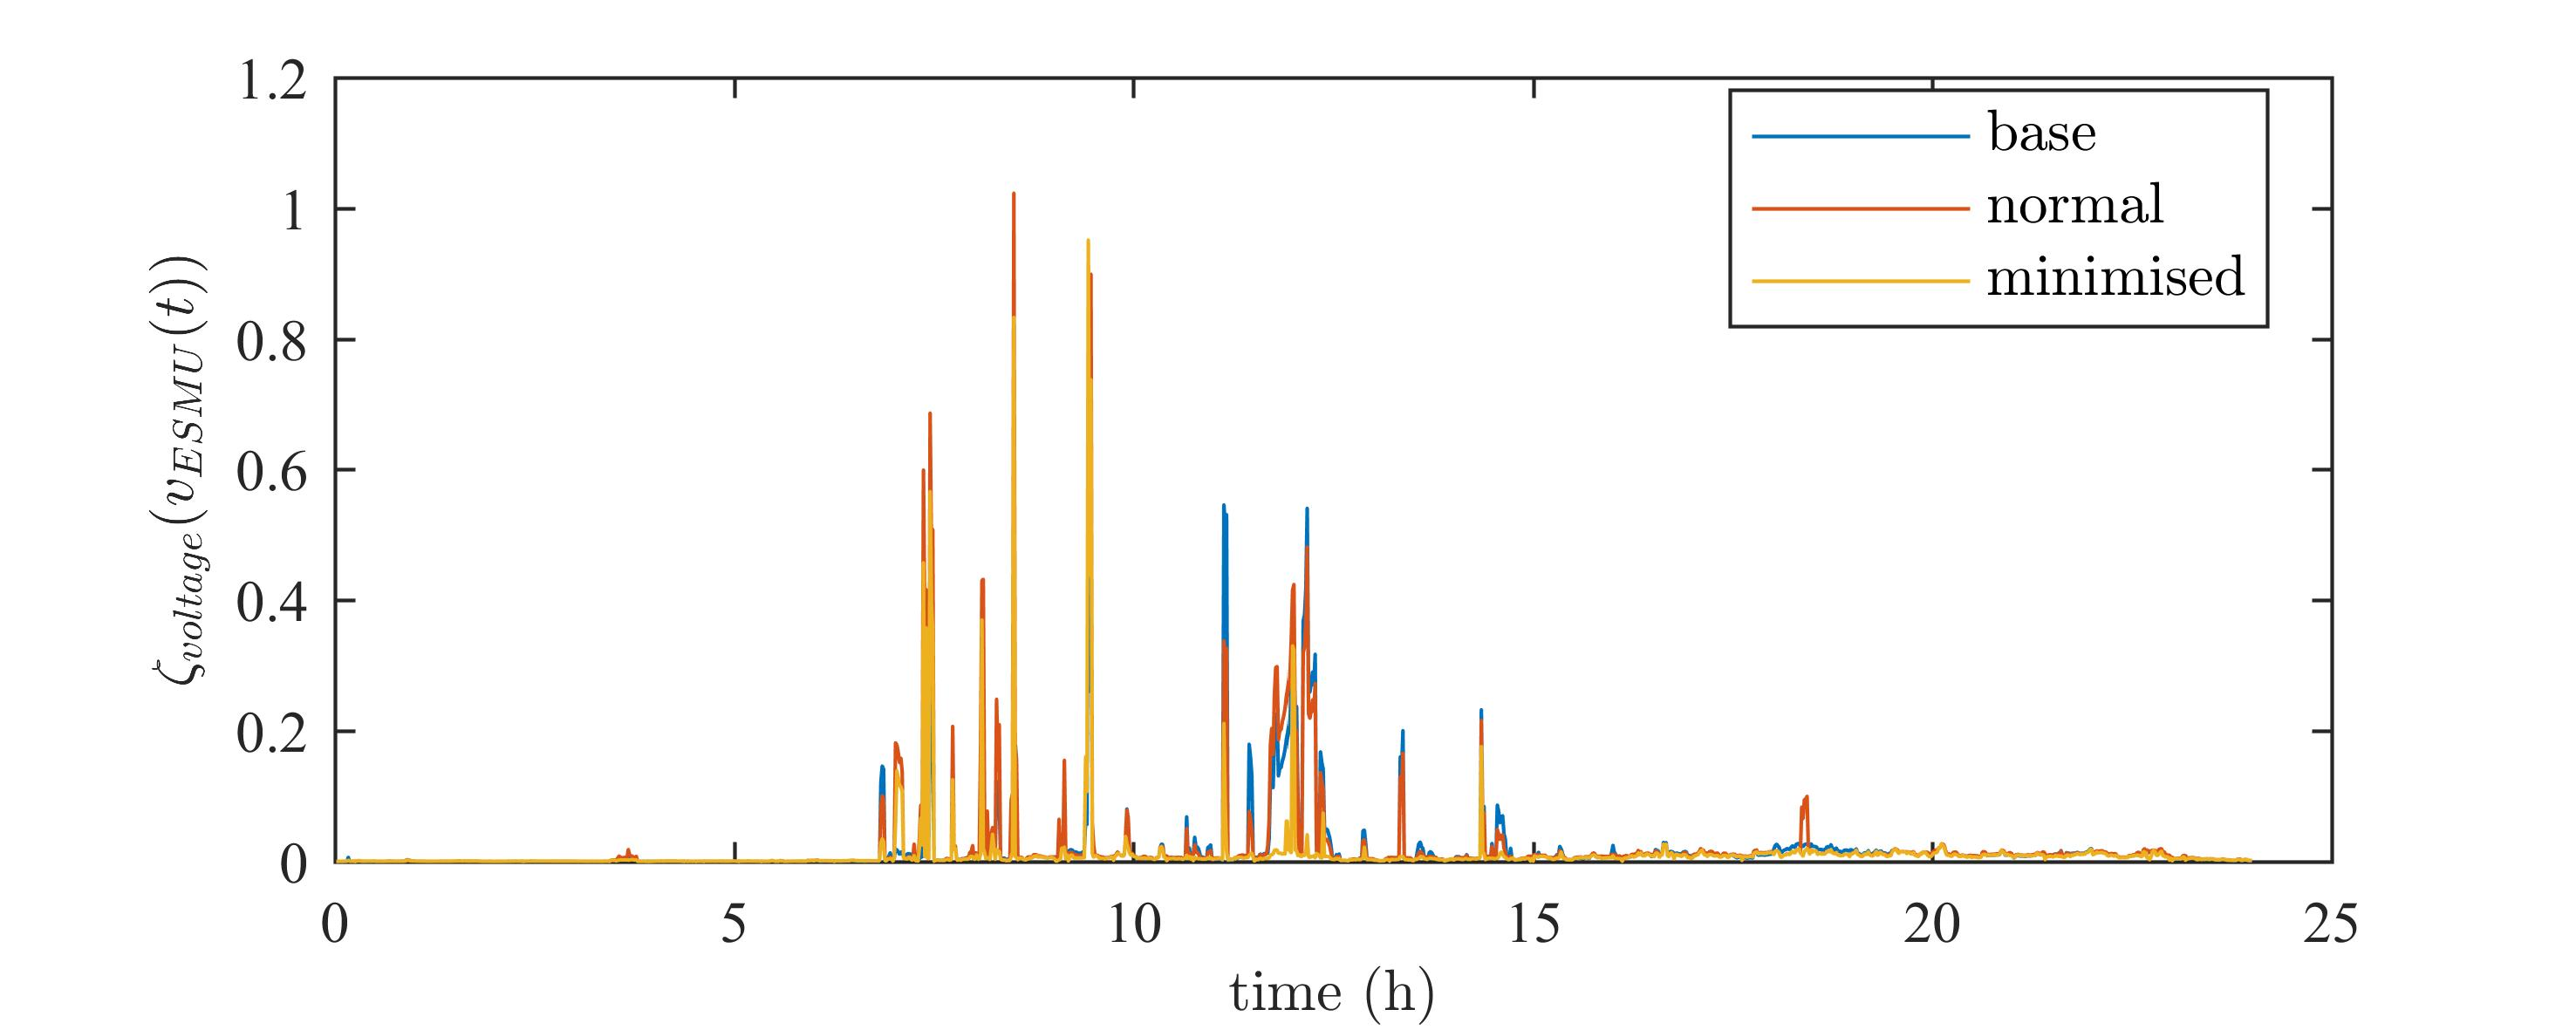
\includegraphics{_chapter1/fig/appendix/ts-esmu-voltages__}}
\caption{Additional ESMU voltage level comparison between base, normal and the case where the ESMU's schedule was adjusted.}
\end{figure}

\begin{figure}\centering
\subfloat[Highest and lowest voltage levels in entire network]{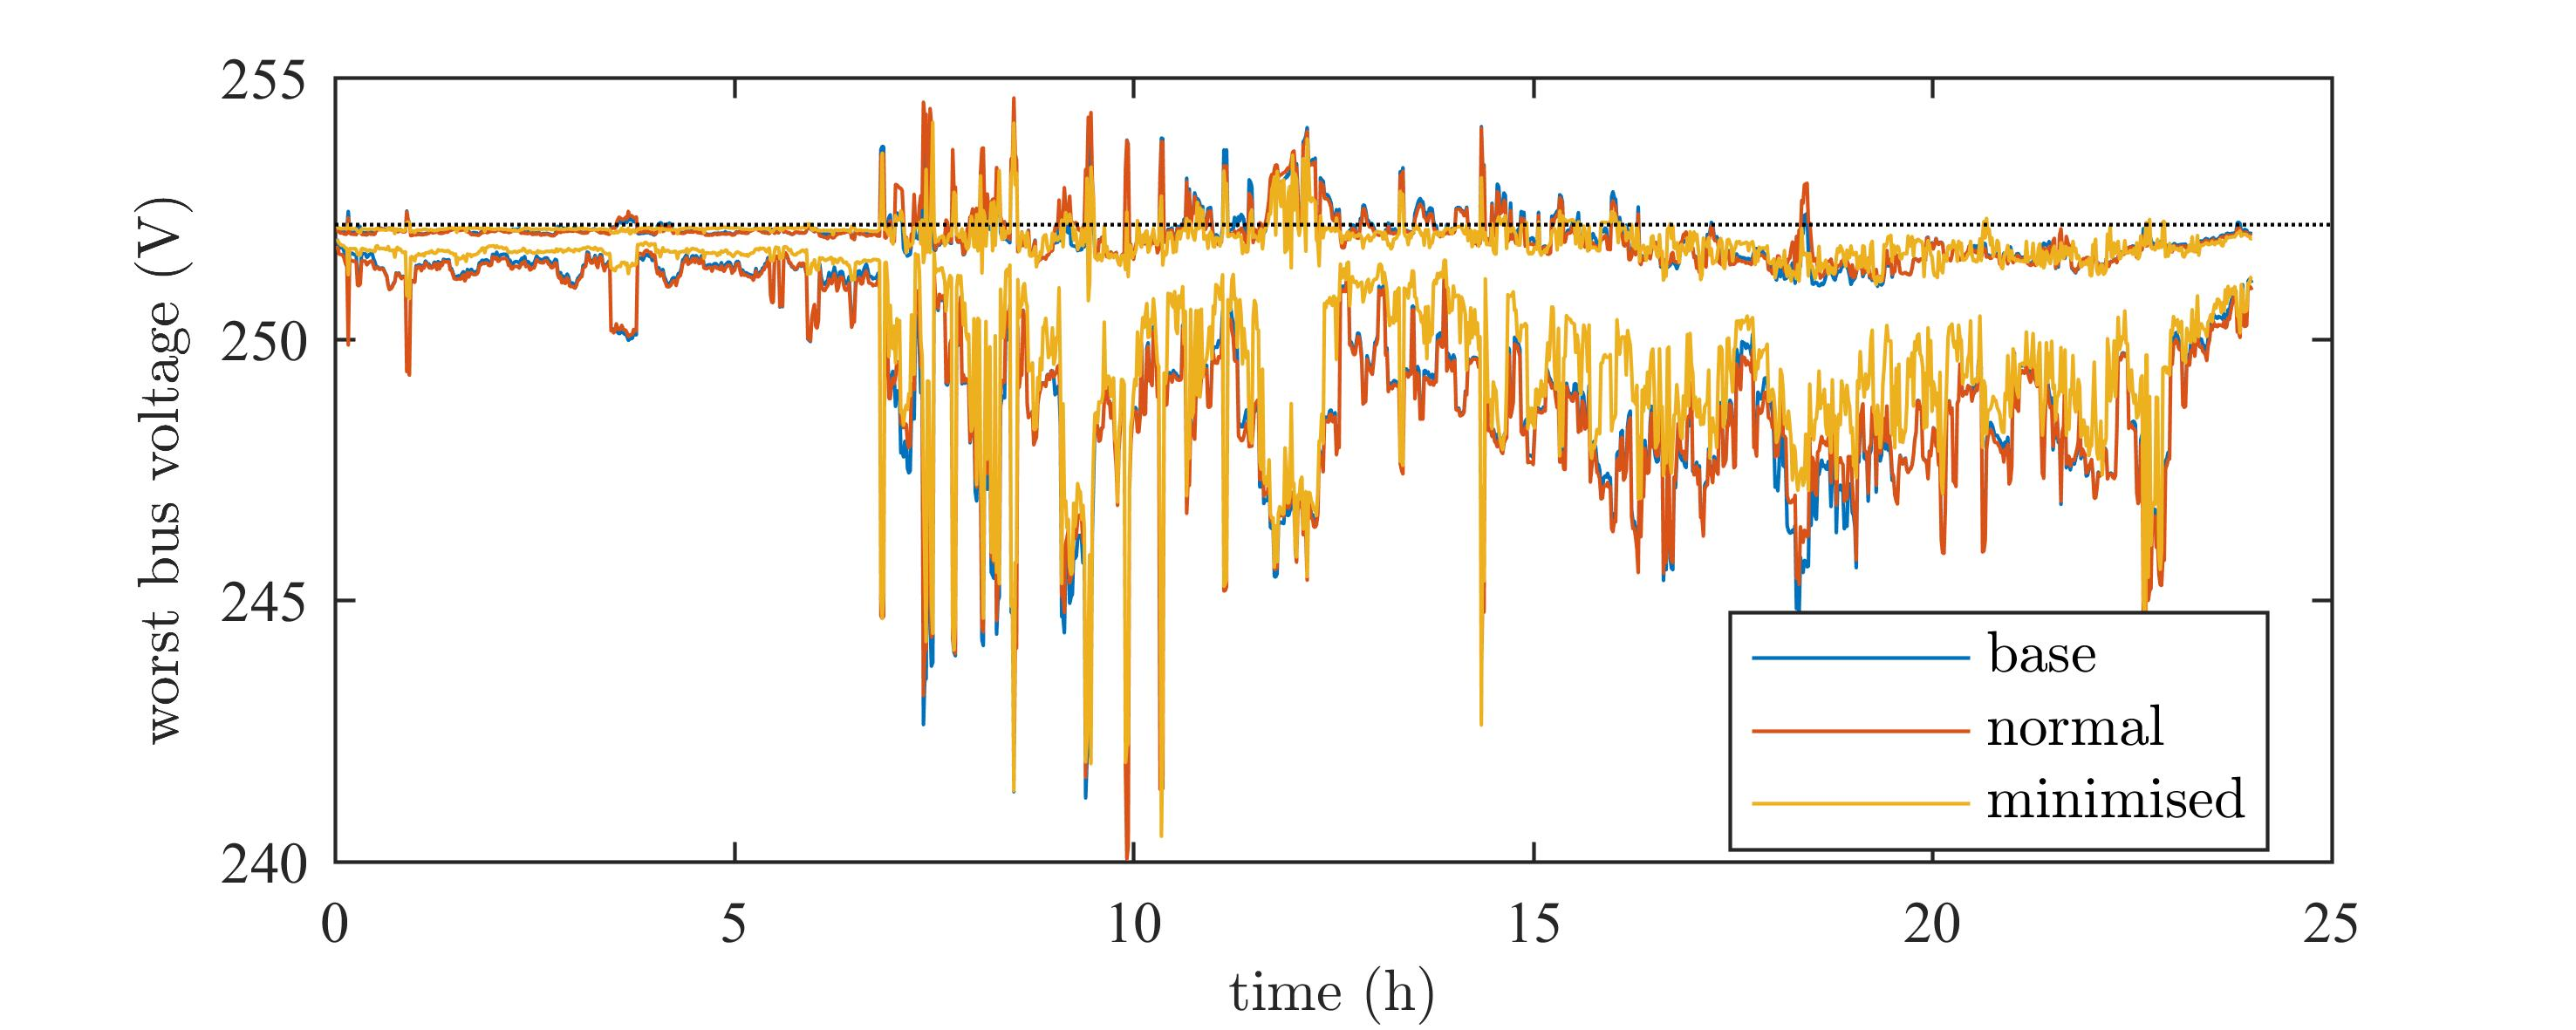
\includegraphics{_chapter1/fig/appendix/ts-all-voltages___}}\\	
\subfloat[Cost associated with highest and lowest voltage levels in entire network]{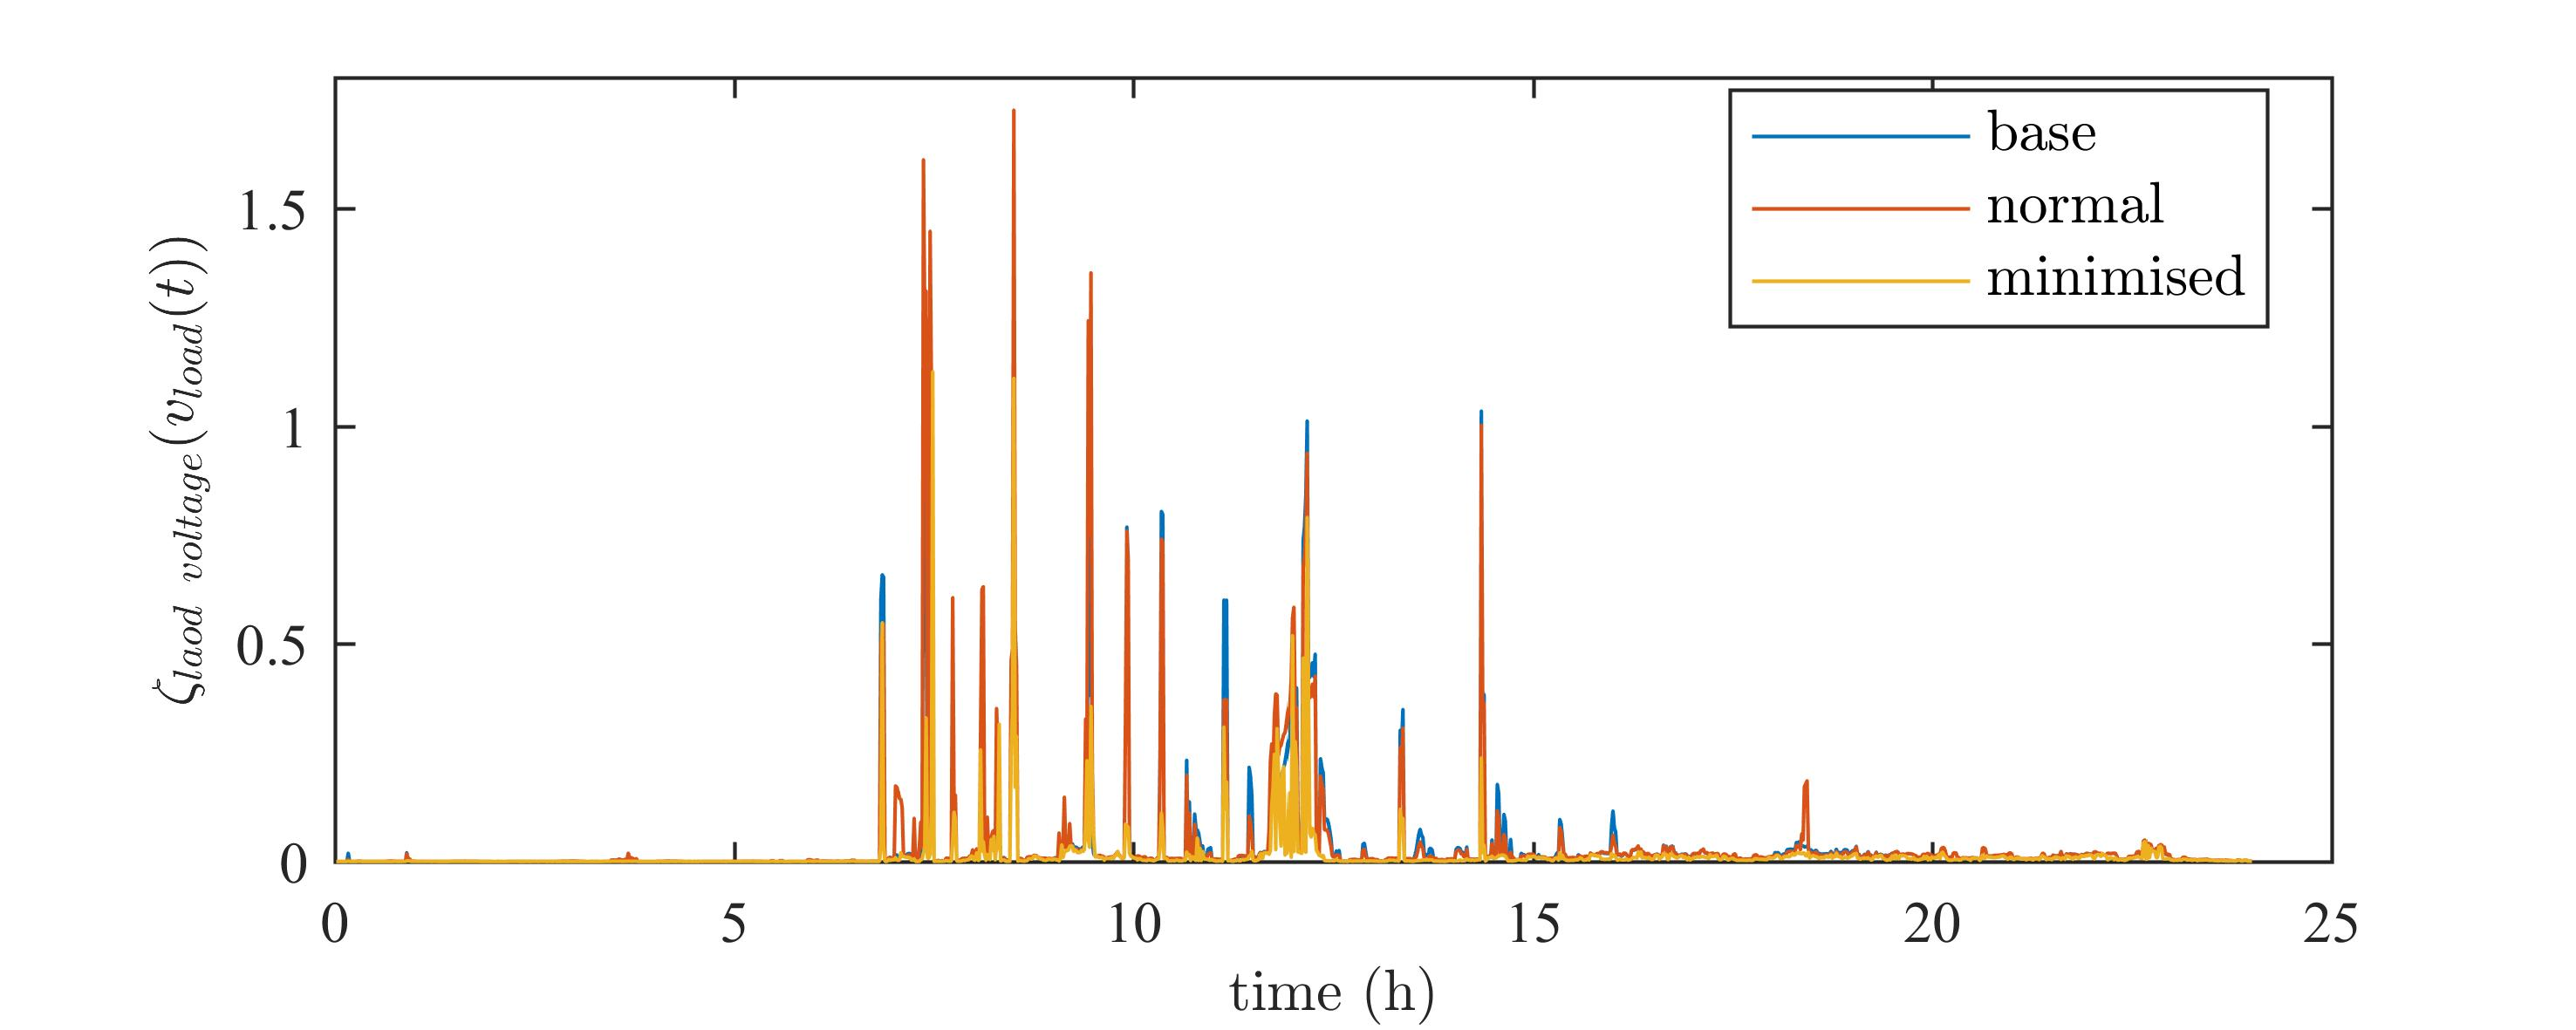
\includegraphics{_chapter1/fig/appendix/ts-all-voltages__}}
\caption{Additional voltage level comparison between base, normal and the case where the ESMU's schedule was adjusted.}
\end{figure}

\begin{figure}\centering
\subfloat[Highest and lowest phase power]{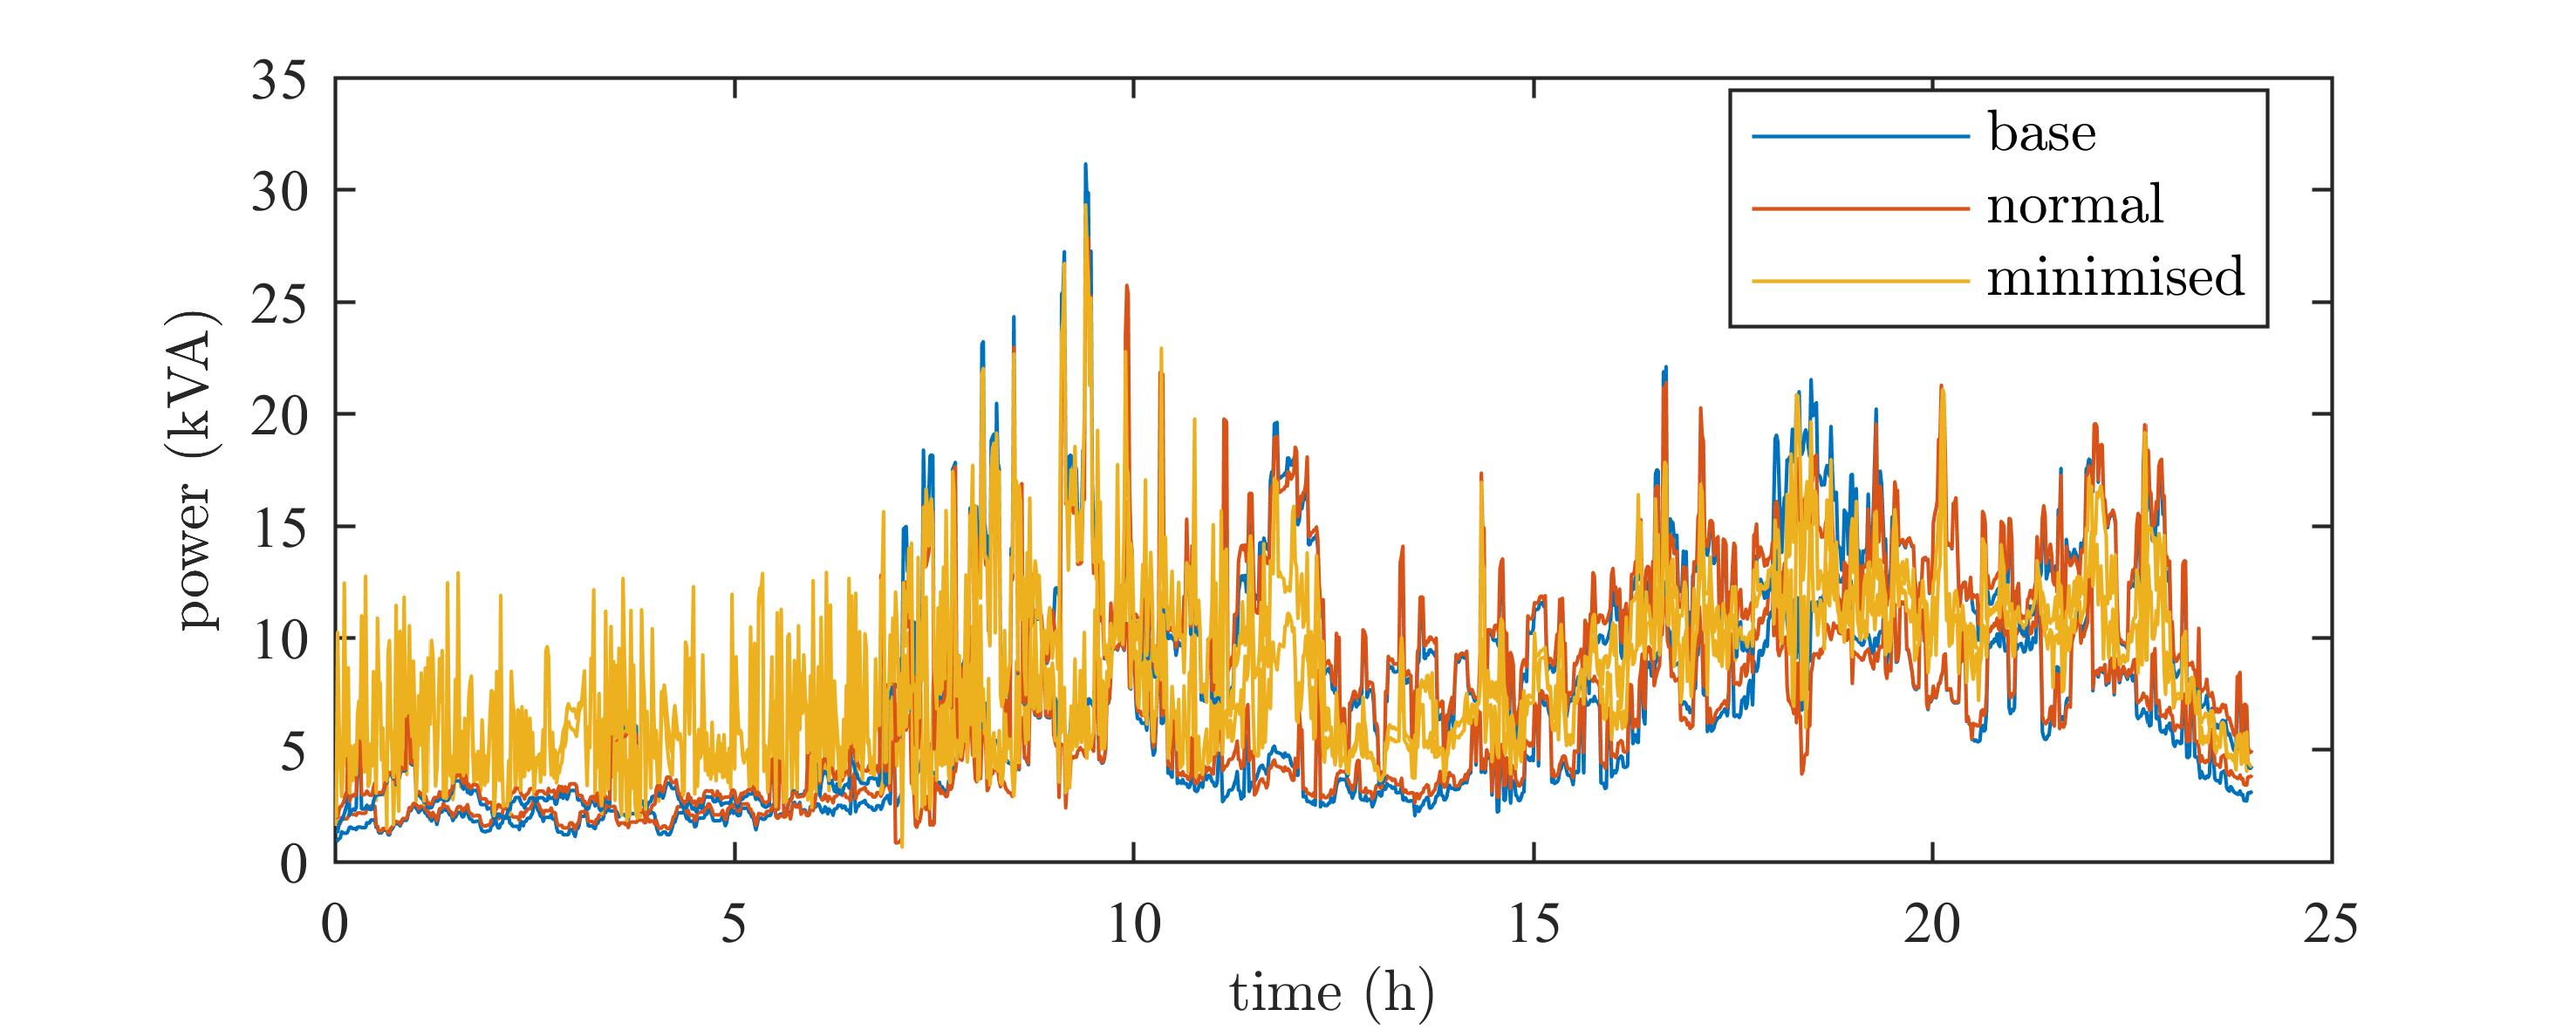
\includegraphics{_chapter1/fig/appendix/ts-phase-unbalance___}}\\	
\subfloat[Phase unbalance cost]{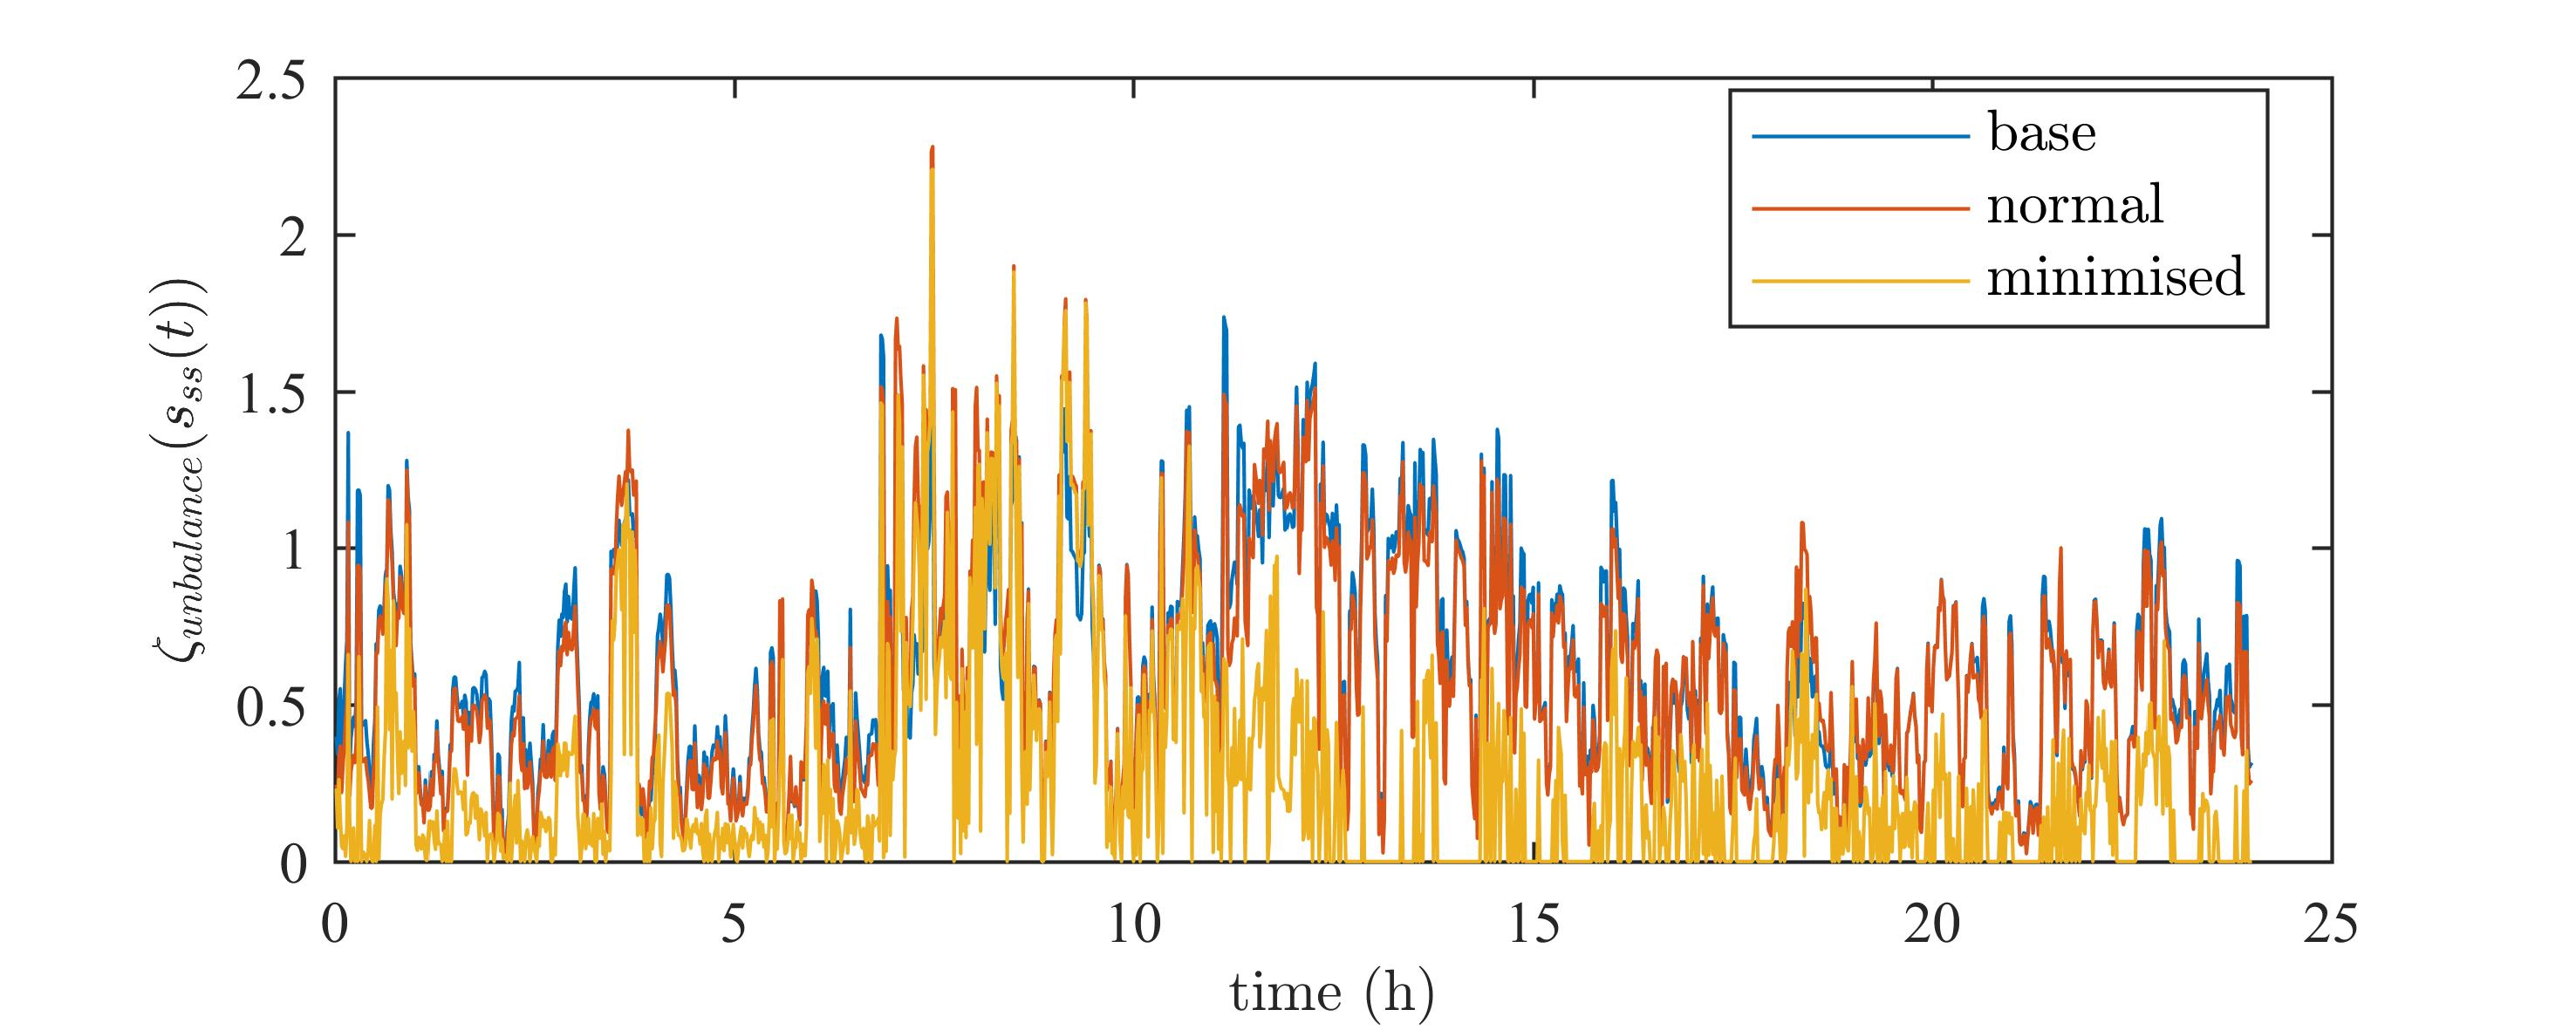
\includegraphics{_chapter1/fig/appendix/ts-phase-unbalance__}}
\caption{Additional phase unbalance cost comparison between base, normal and the case where the ESMU's schedule was adjusted.}
\end{figure}

\begin{figure}\centering
\subfloat[Network load]{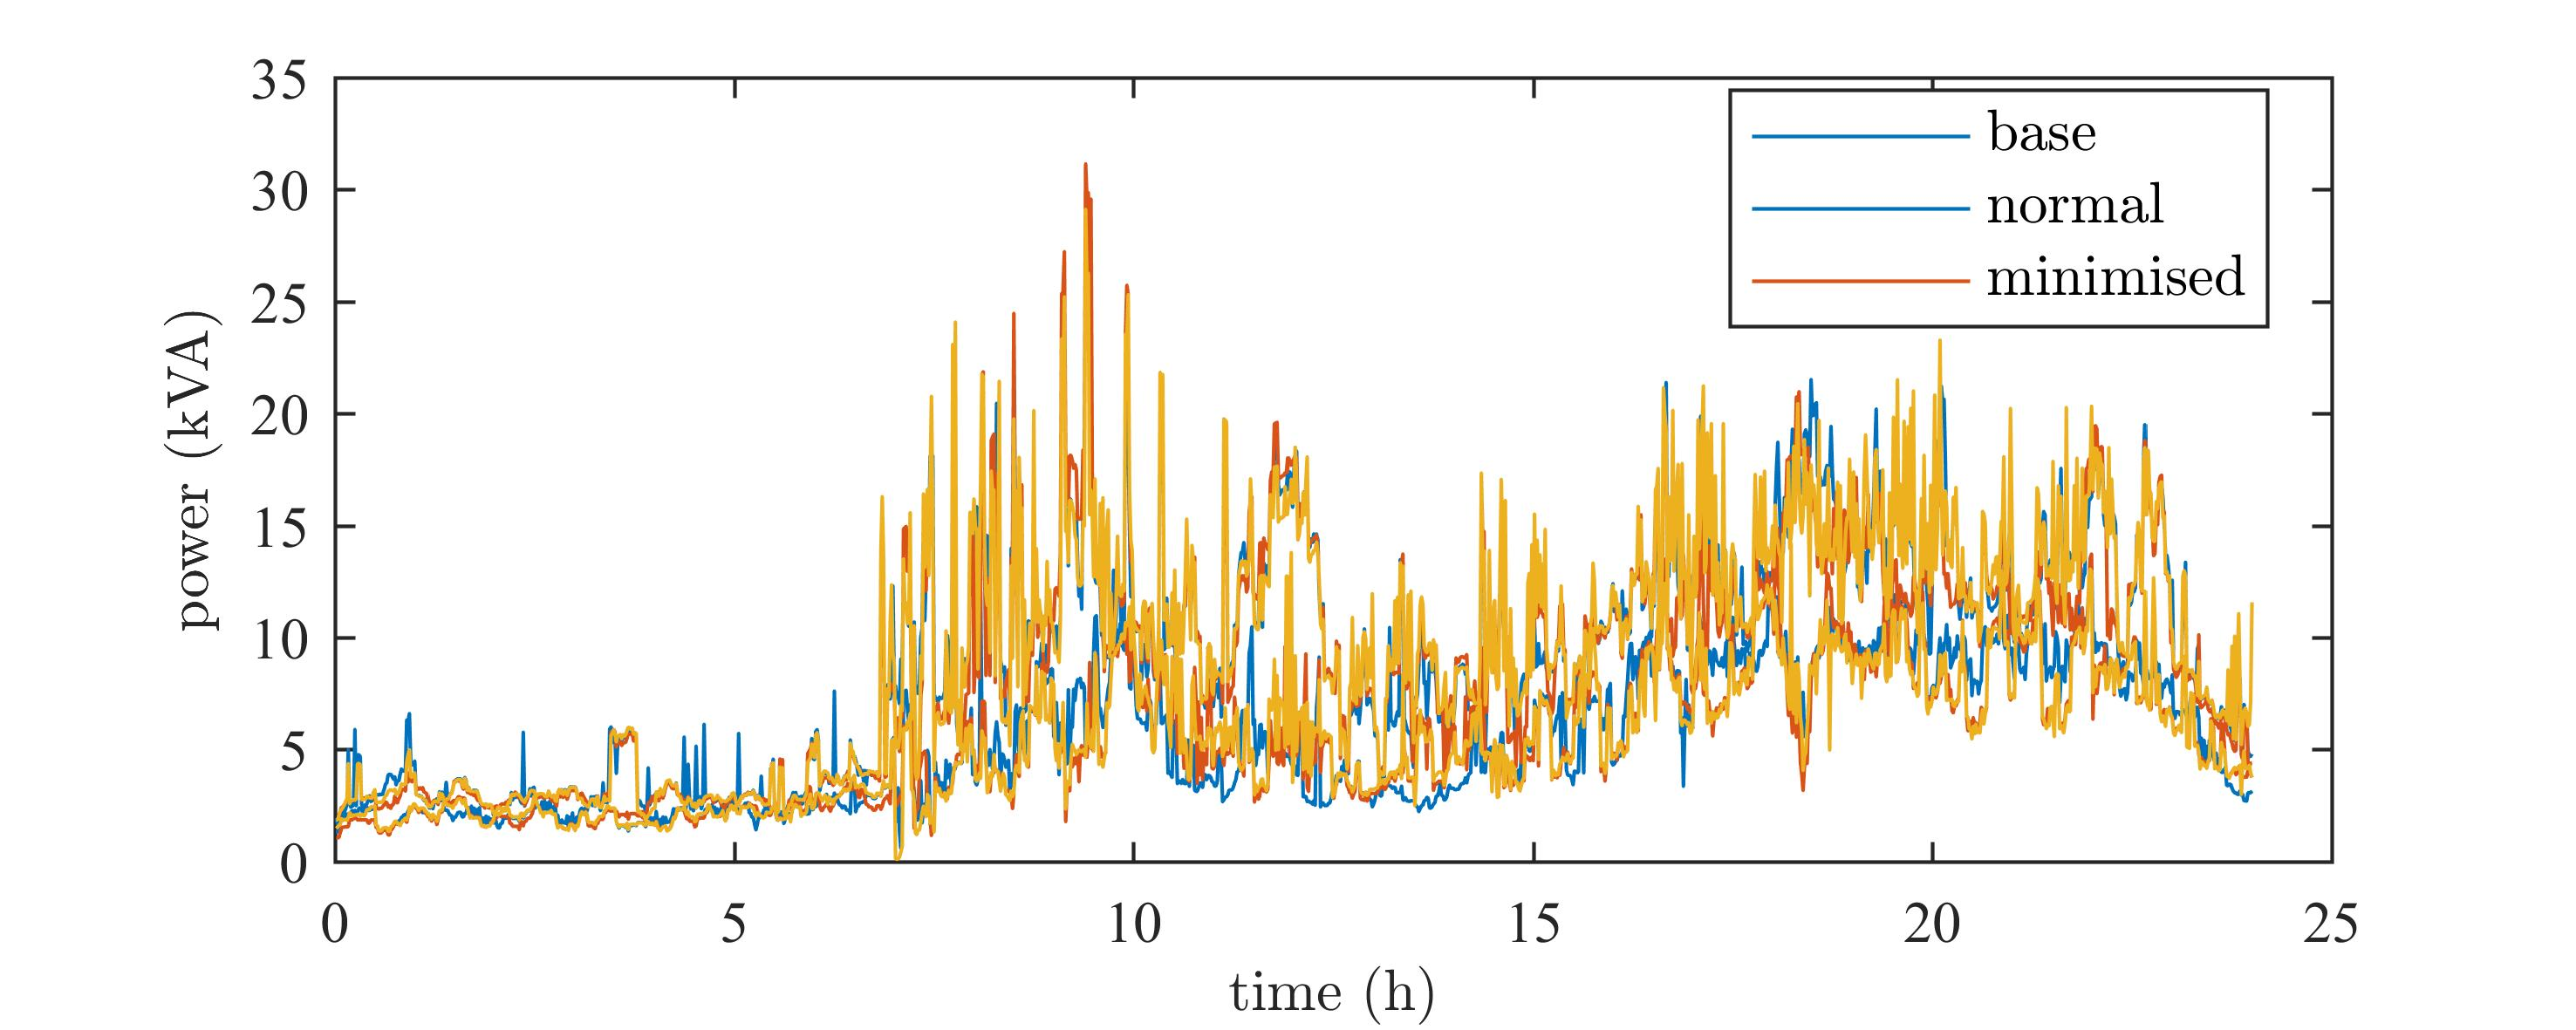
\includegraphics{_chapter1/fig/appendix/ts-power-factor___}}\\	
\subfloat[Power factor]{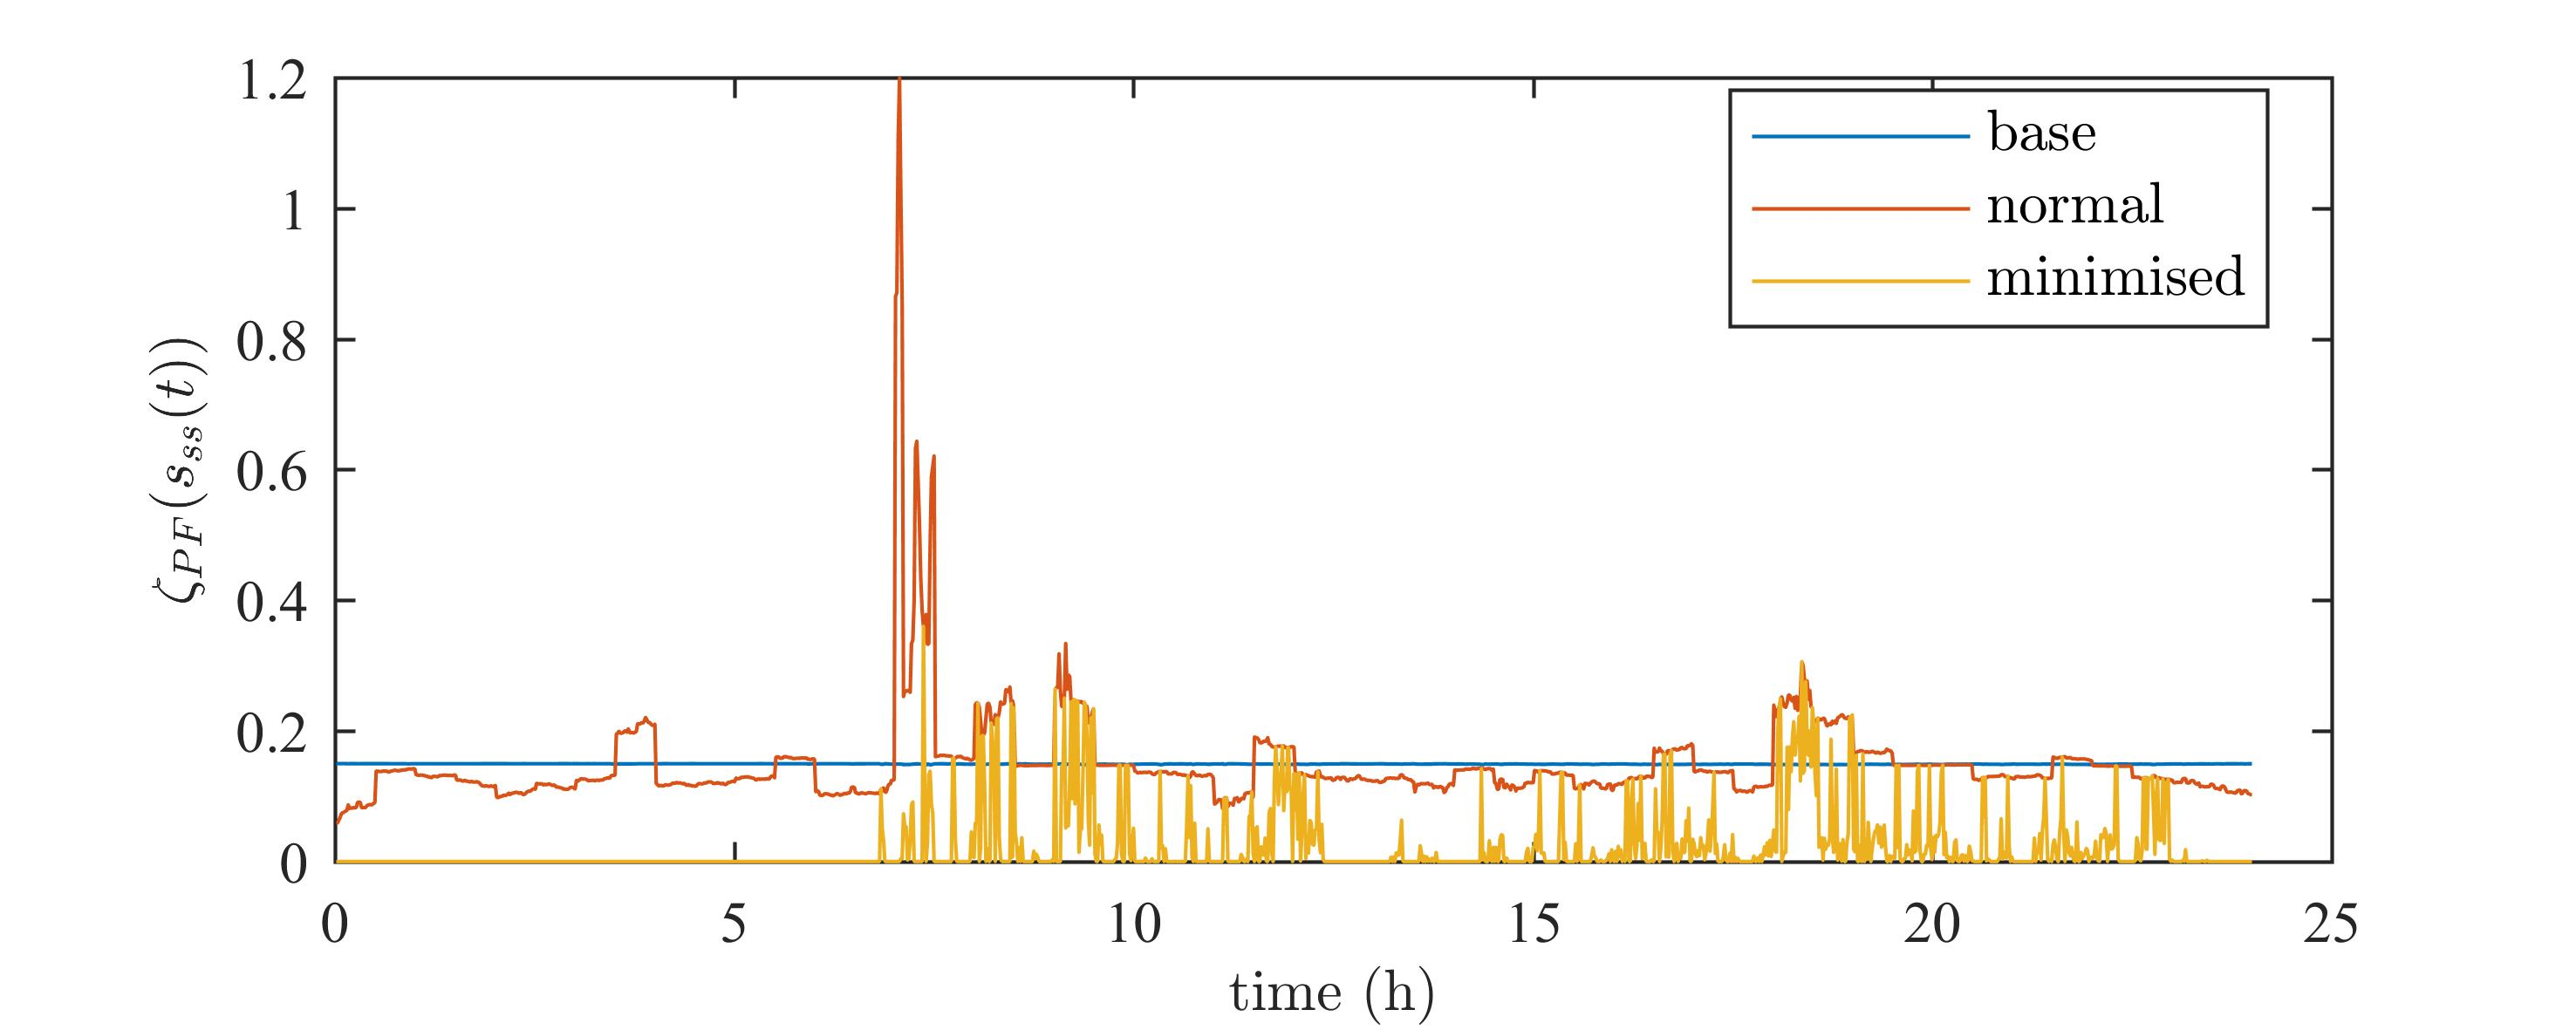
\includegraphics{_chapter1/fig/appendix/ts-power-factor__}}
\caption{Additional power factor cost comparison between base, normal and the case where the ESMU's schedule was adjusted.}
\end{figure}

\begin{figure}\centering
\subfloat[Utilisation of the substation fuse]{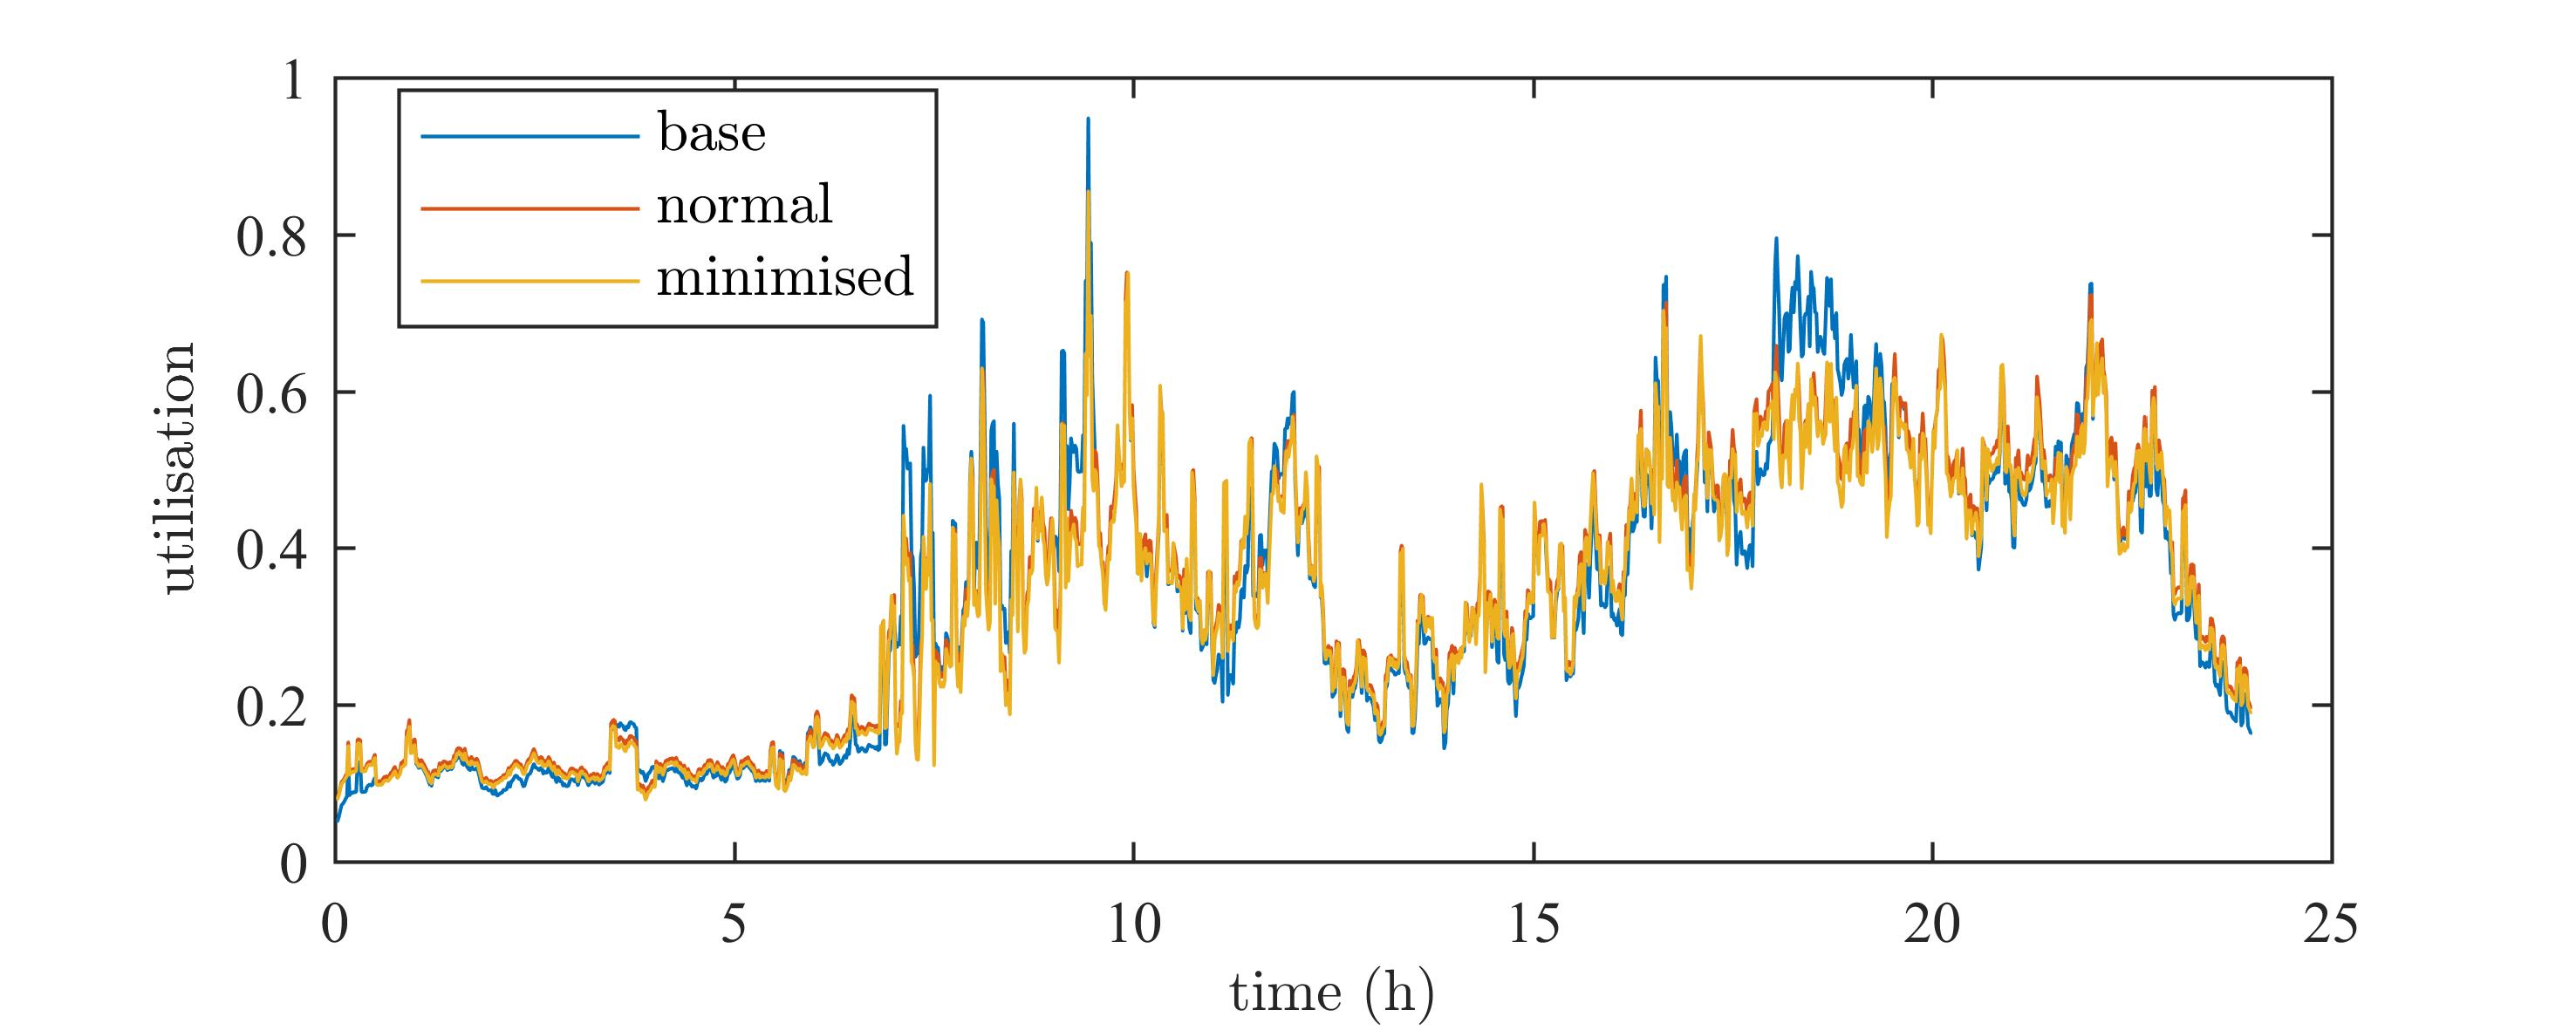
\includegraphics{_chapter1/fig/appendix/ts-fuse-utilisation___}}\\	
\subfloat[Cost associated with the utilisation of the substation fuse]{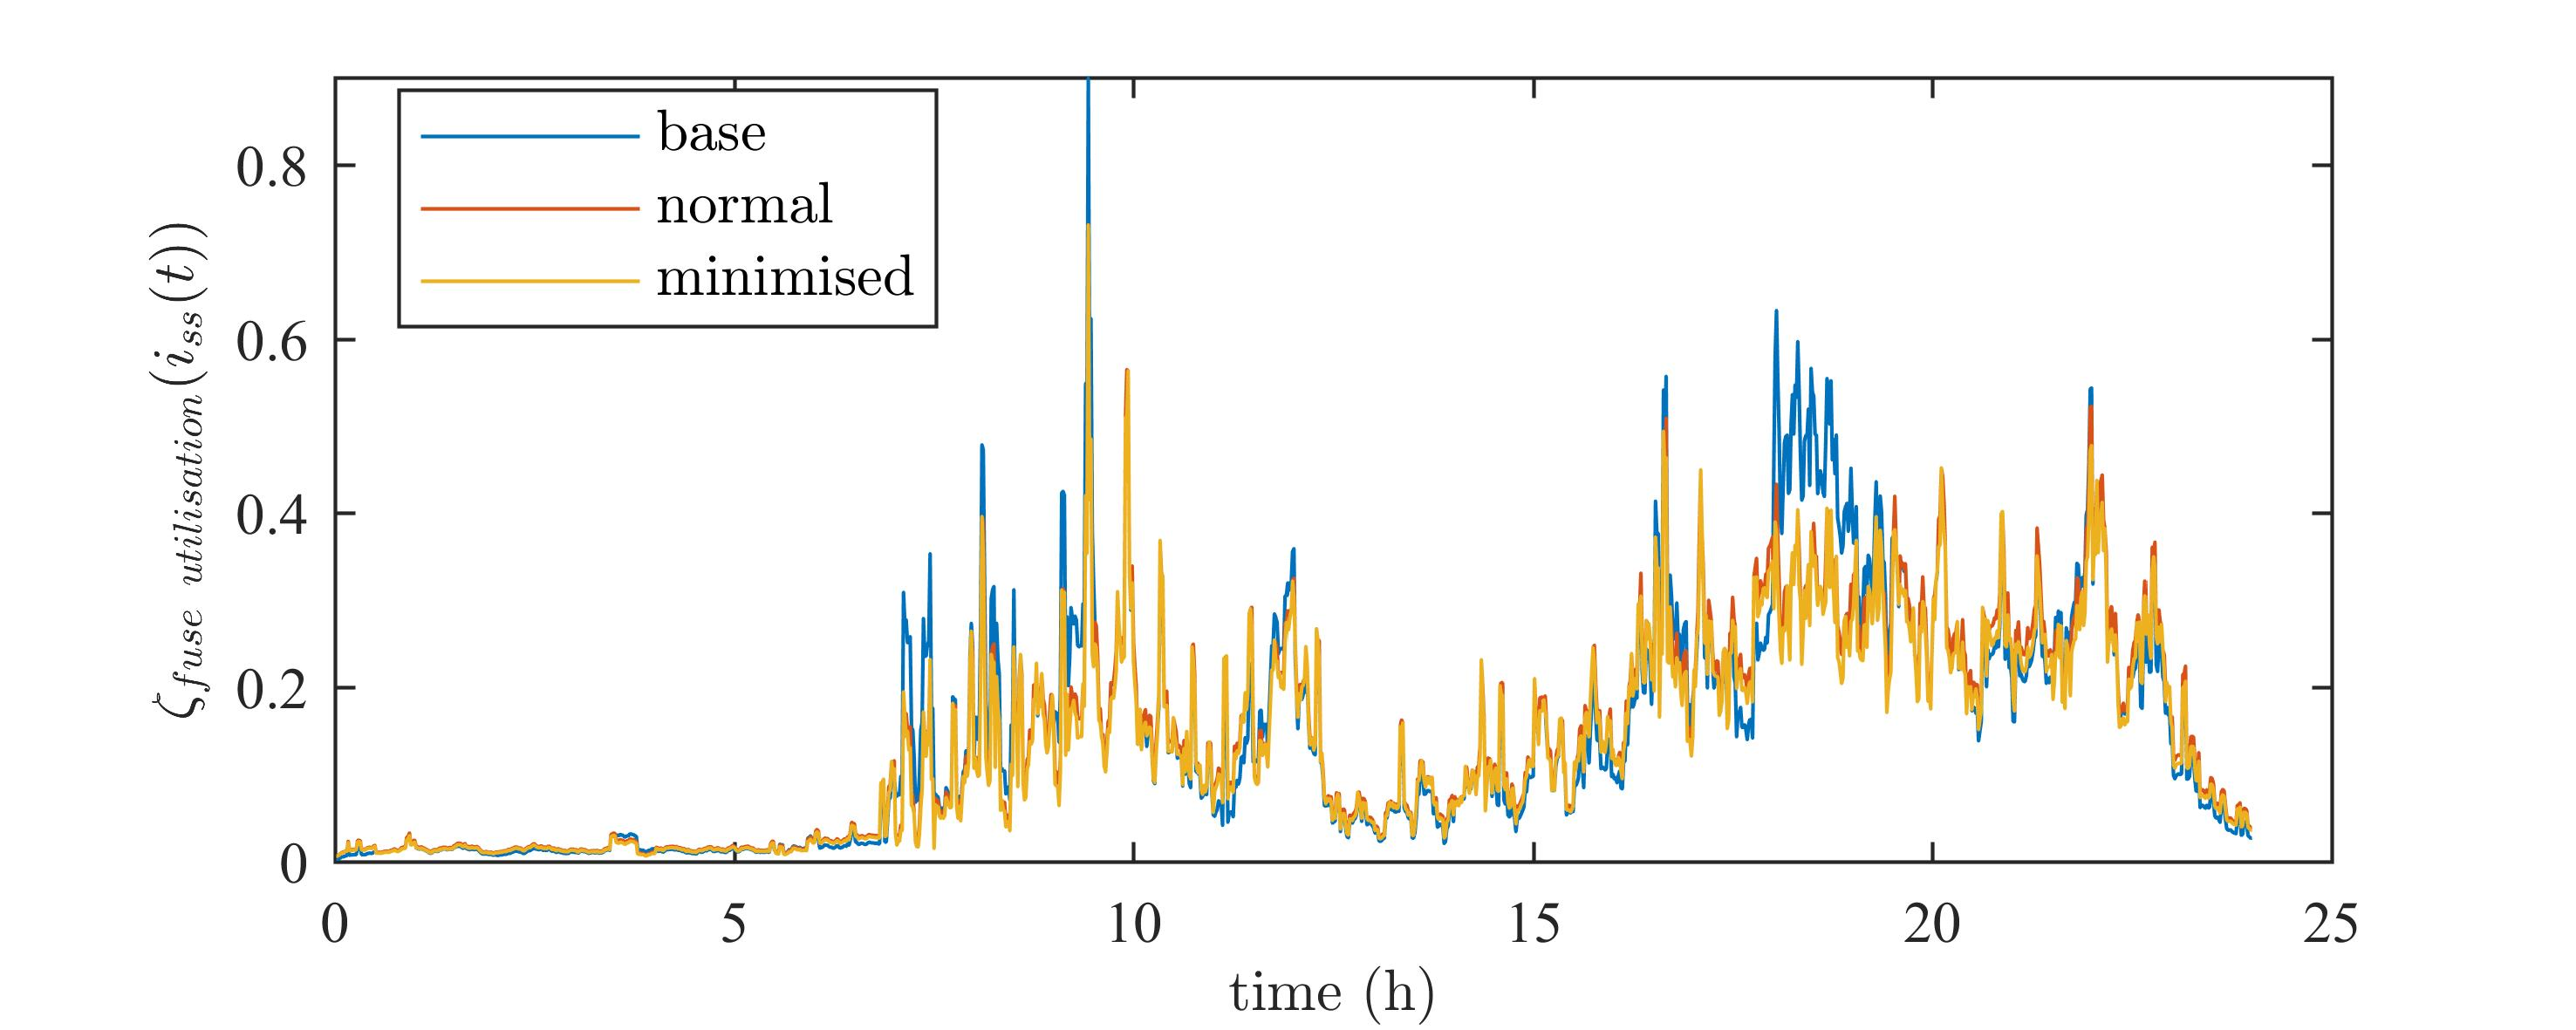
\includegraphics{_chapter1/fig/appendix/ts-fuse-utilisation__}}
\caption{Additional comparison of the substation fuse utilisation between base, normal and the case where the ESMU's schedule was adjusted.}
\end{figure}

\begin{figure}\centering
\subfloat[The highest line utilisation of any line in the entire network]{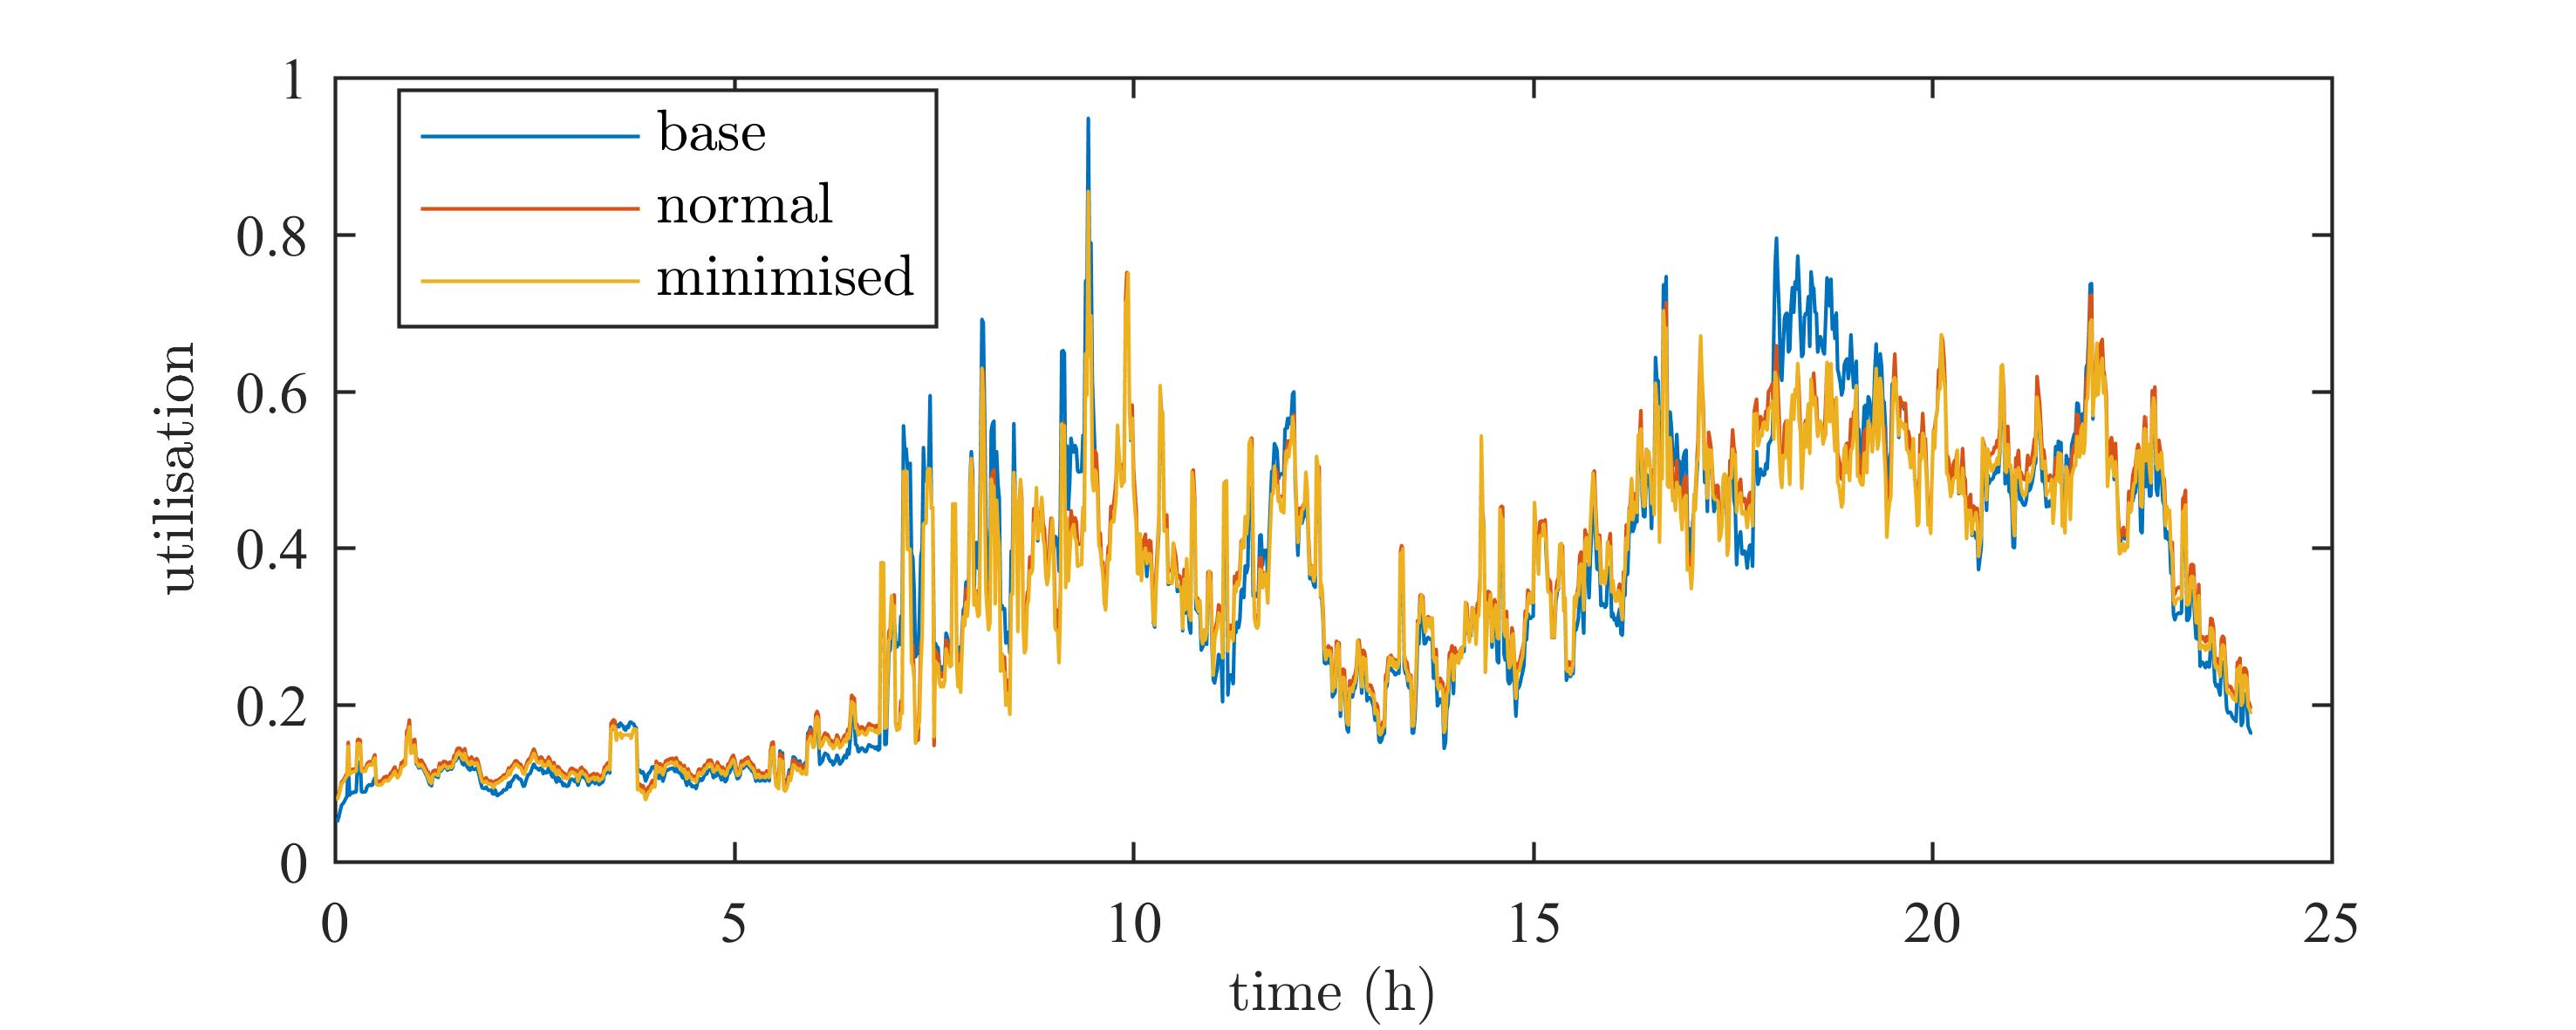
\includegraphics{_chapter1/fig/appendix/ts-all-line-utilisation___}}\\	
\subfloat[The highest cost associated to the highest line utilisation of any line in the entire network]{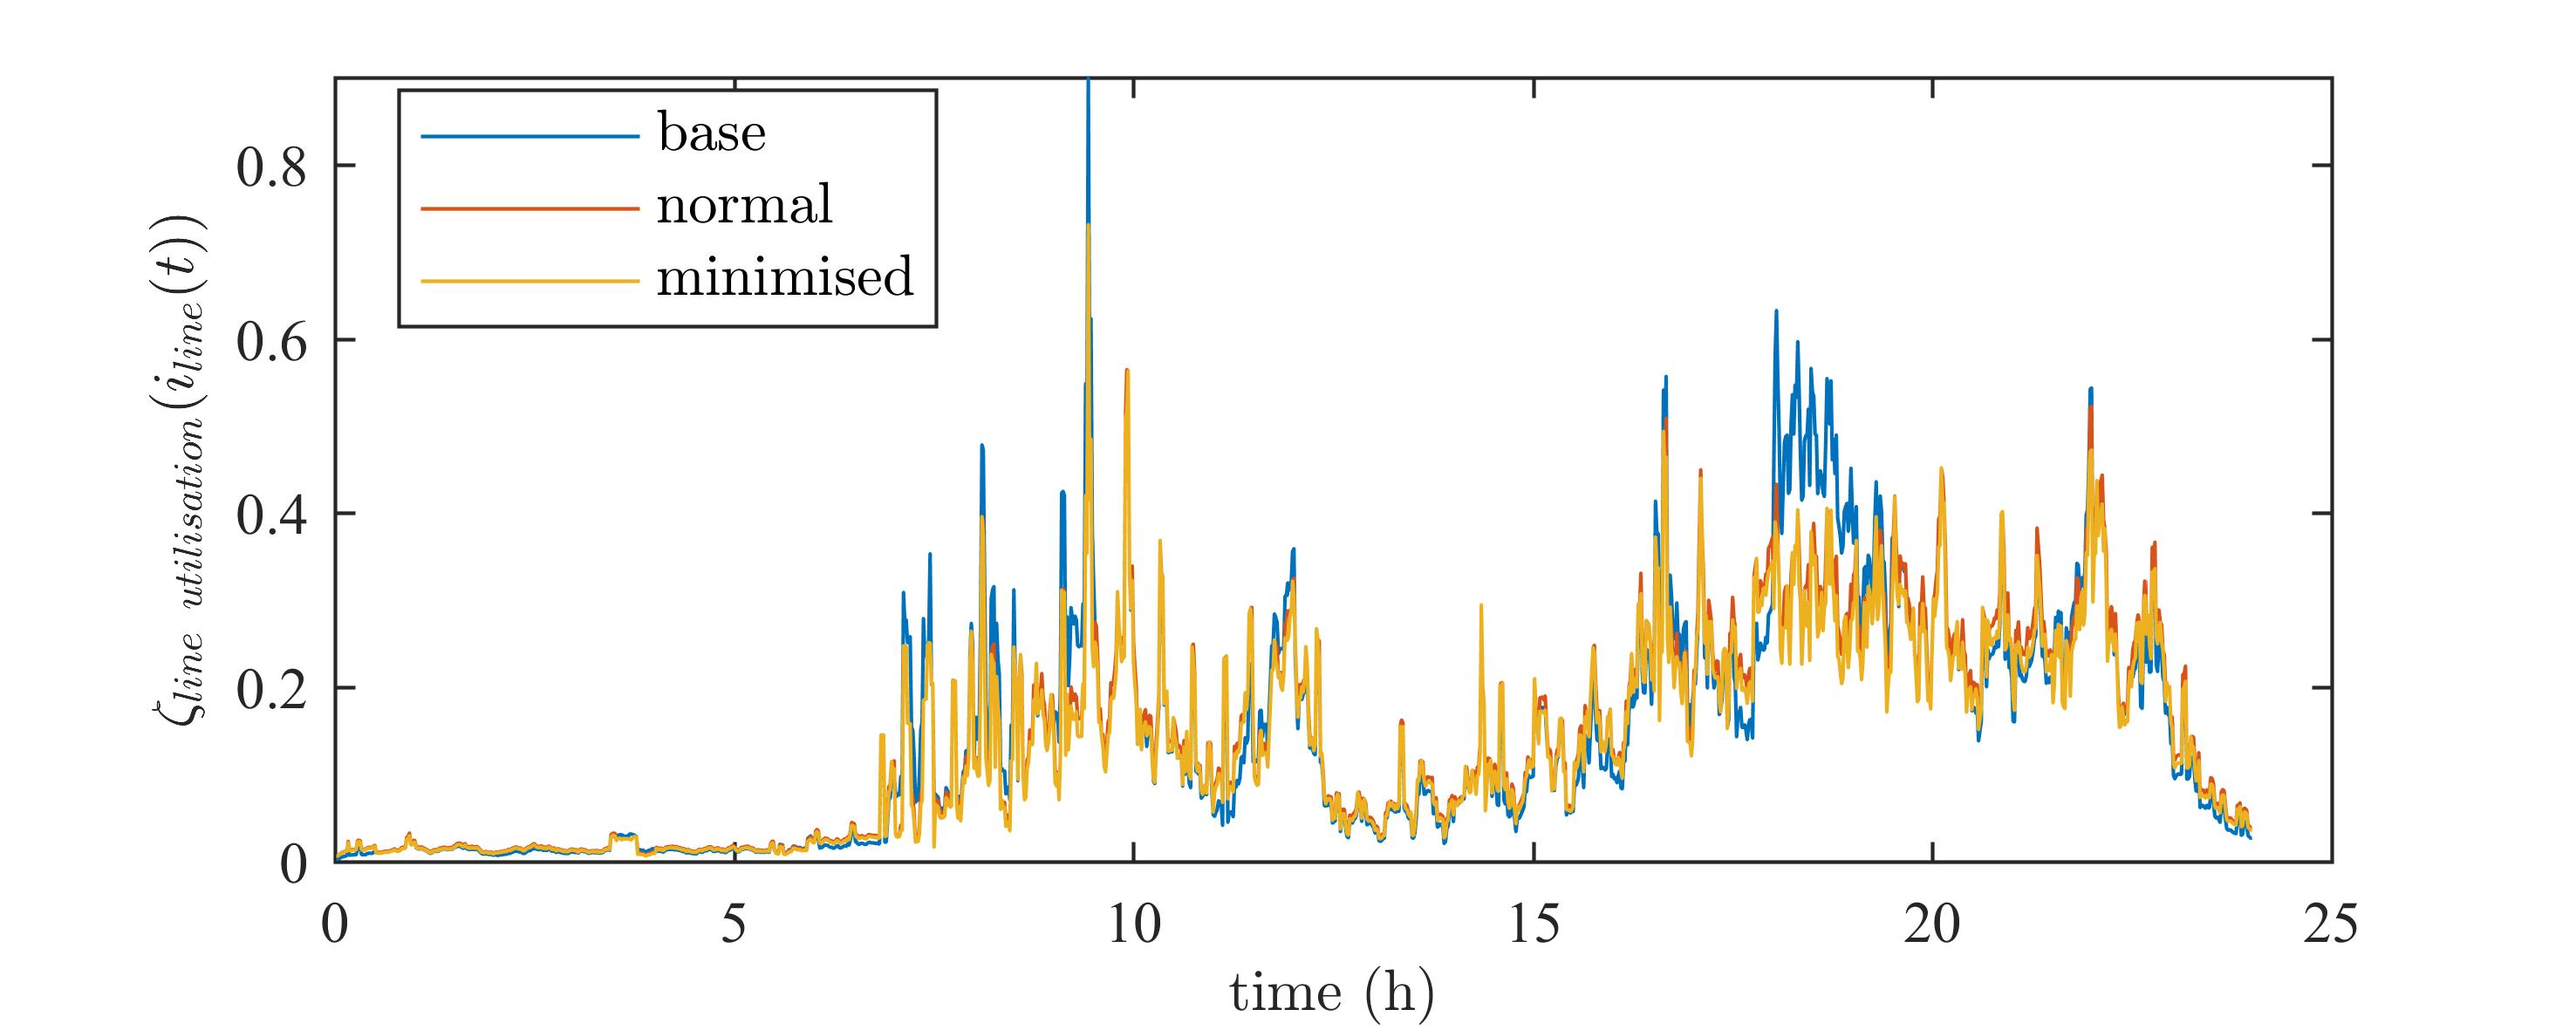
\includegraphics{_chapter1/fig/appendix/ts-all-line-utilisation__}}
\caption{Additional line utilisation comparison between base, normal and the case where the ESMU's schedule was adjusted.}
\end{figure}

\begin{figure}\centering
\subfloat[Distribution losses]{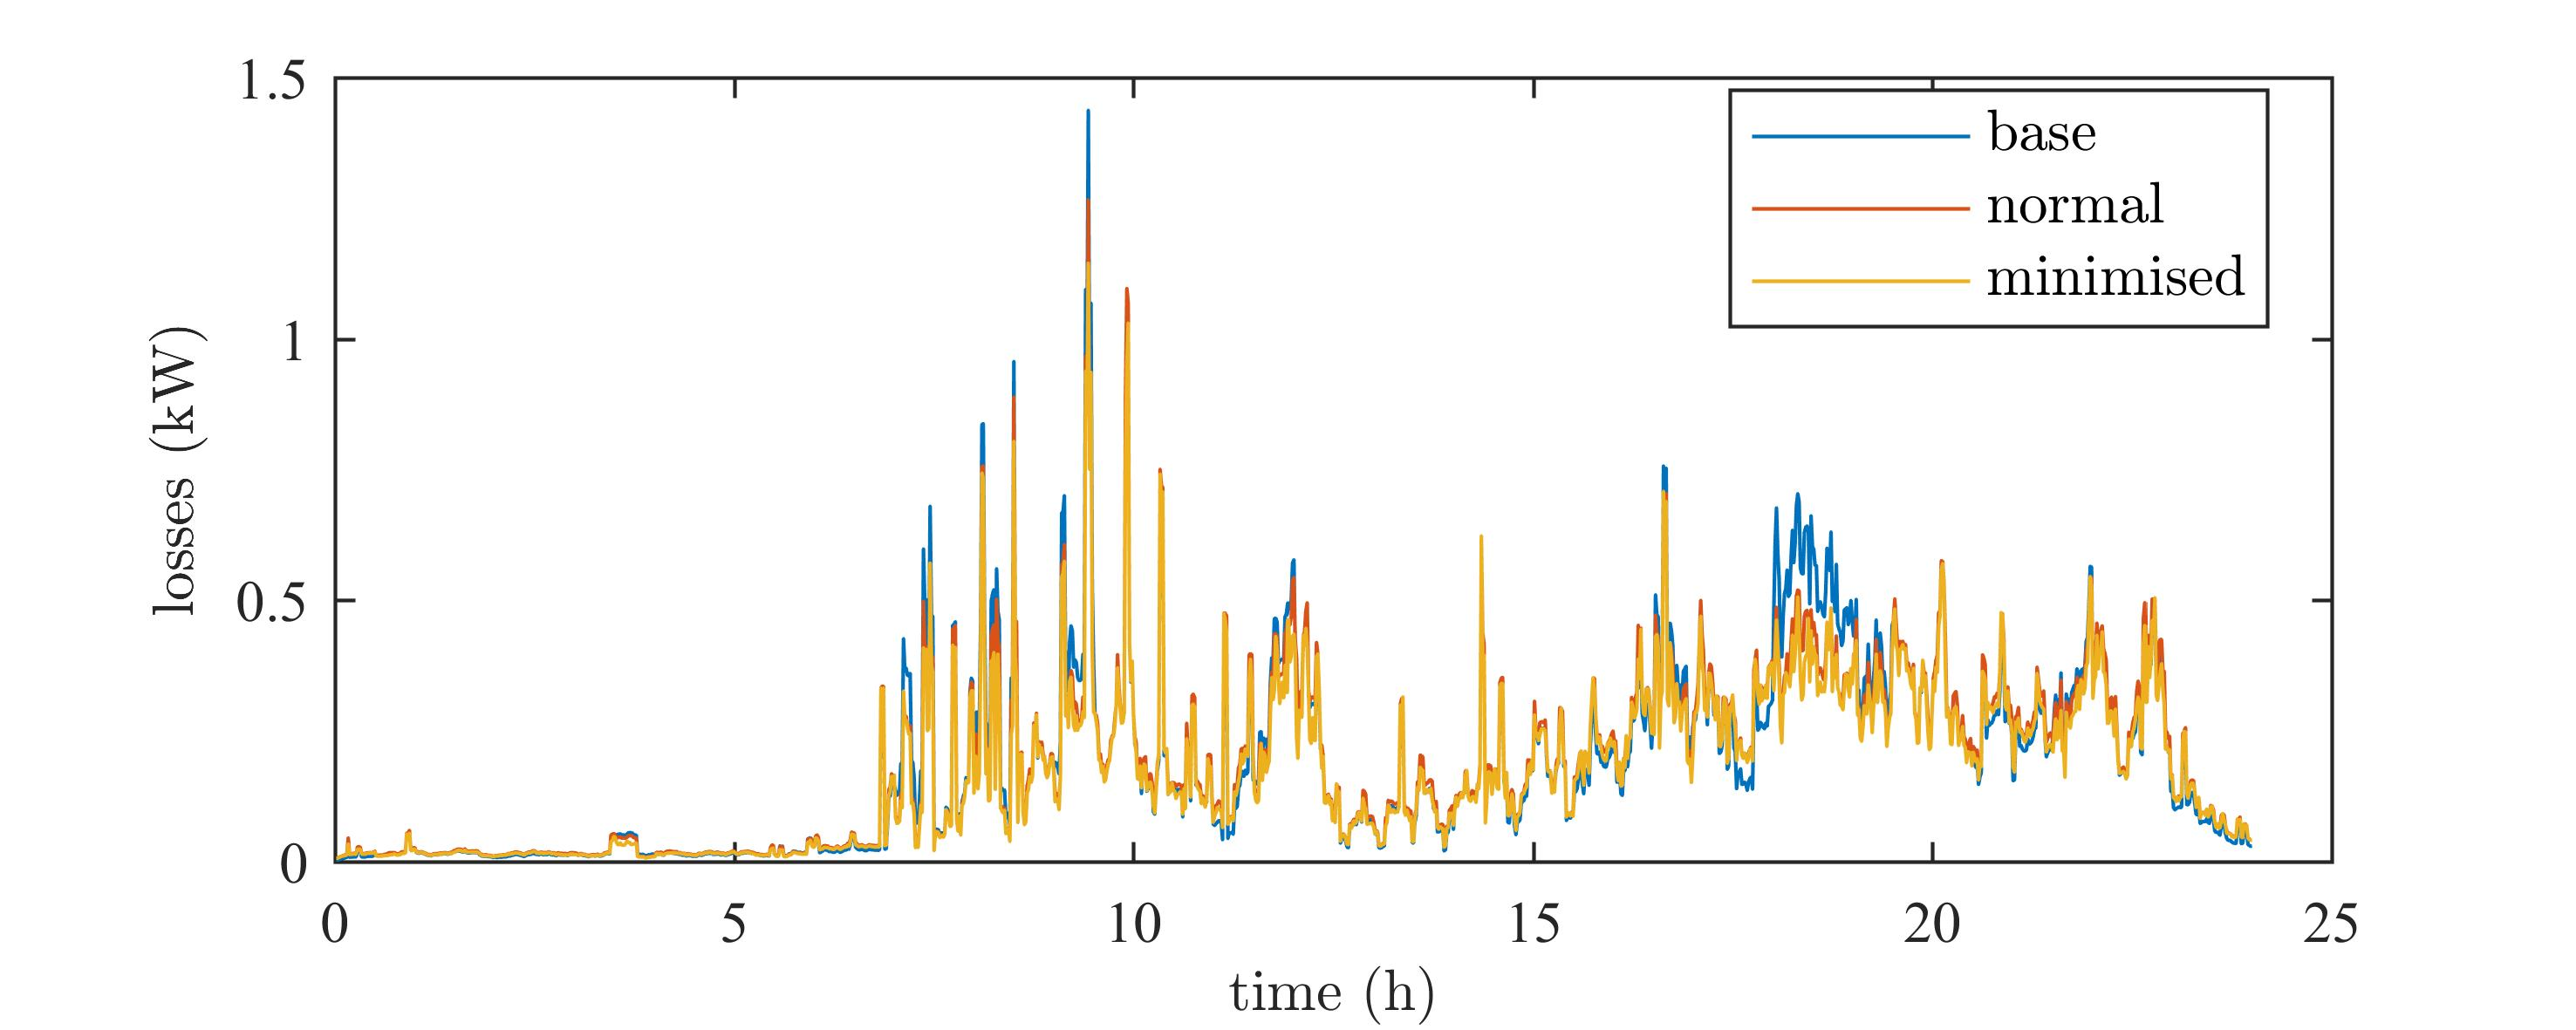
\includegraphics{_chapter1/fig/appendix/ts-losses___}}\\	
\subfloat[Cost associated to distribution losses]{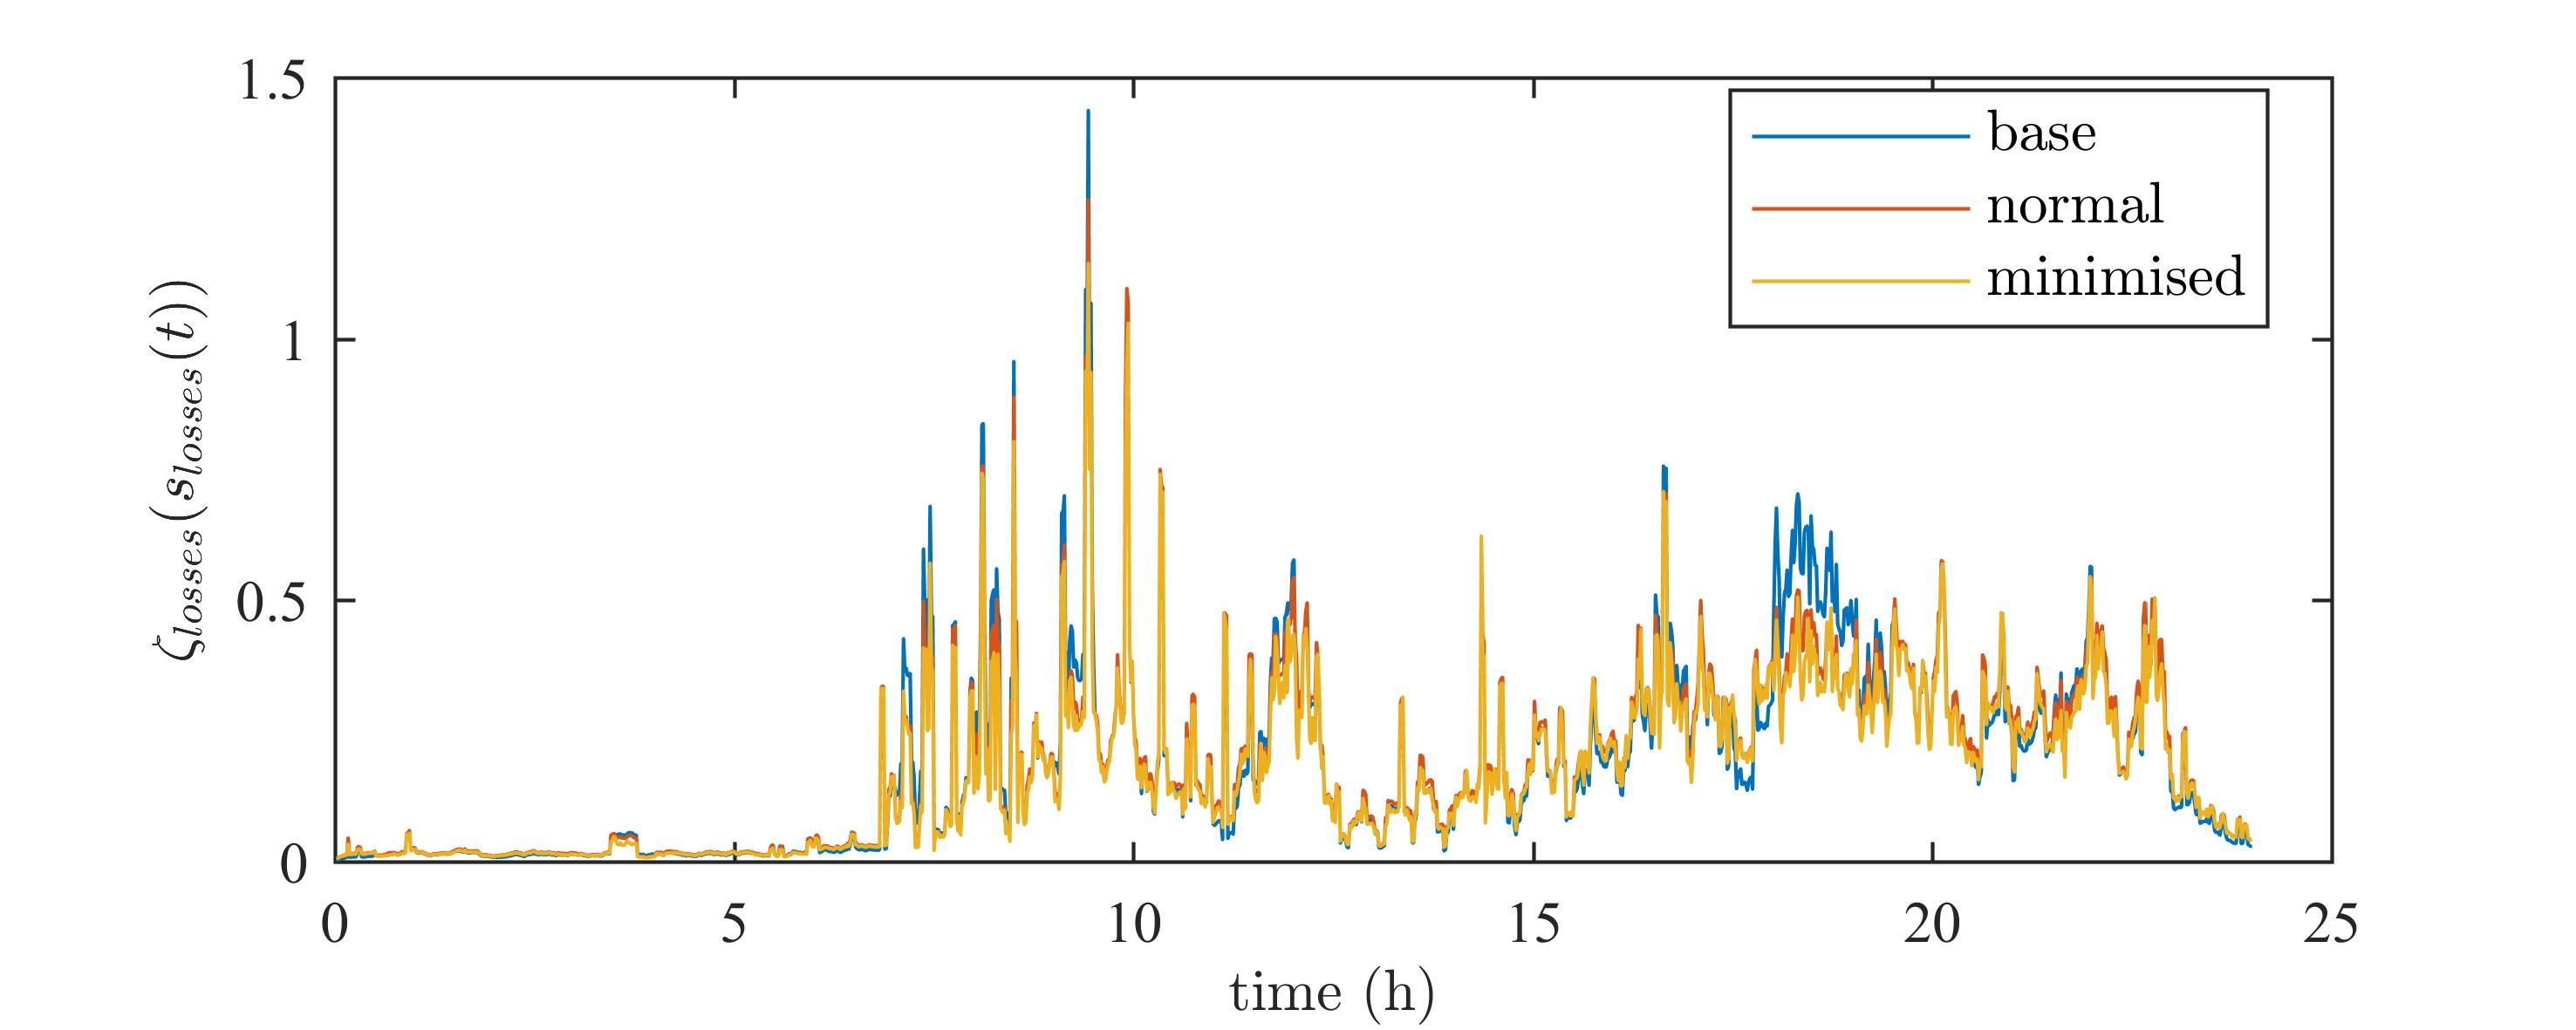
\includegraphics{_chapter1/fig/appendix/ts-losses__}}
\caption{Additional comparison of distribution loss cost between base, normal and the case where the ESMU's schedule was adjusted.}
\end{figure}